\chapter{Design}
\label{sec:design}

% Ist das zentrale Kapitel der Arbeit. Hier werden das Ziel sowie die
% eigenen Ideen, Wertungen, Entwurfsentscheidungen vorgebracht. Es kann
% sich lohnen, verschiedene Möglichkeiten durchzuspielen und dann
% explizit zu begründen, warum man sich für eine bestimmte entschieden
% hat. Dieses Kapitel sollte - zumindest in Stichworten - schon bei den
% ersten Festlegungen eines Entwurfs skizziert werden.
% Es wird sich aber in einer normal verlaufenden
% Arbeit dauernd etwas daran ändern. Das Kapitel darf nicht zu
% detailliert werden, sonst langweilt sich der Leser. Es ist sehr
% wichtig, das richtige Abstraktionsniveau zu finden. Beim Verfassen
% sollte man auf die Wiederverwendbarkeit des Textes achten.

% Plant man eine Veröffentlichung aus der Arbeit zu machen, können von
% diesem Kapitel Teile genommen werden. Das Kapitel wird in der Regel
% wohl mindestens 8 Seiten haben, mehr als 20 können ein Hinweis darauf
% sein, daß das Abstraktionsniveau verfehlt wurde.

%\ldots design \ldots

%\todo{write design}
This chapter will present a shielding layer design to mitigate the vulnerabilities found in security analysis over OCI runtime interface (refer to Section~\ref{sec:security_analyse_oci_summary}). The shielding layer consists of the remote attestation and provisioning infrastructure, CVM runtime measurement manager, the EXEC request checker, 
guest process STDIO protector, system call interceptor, and guest log manager. The remote attestation and provisioning infrastructure offers a secure mechanism for managing and deploying secrets. This mechanism can be employed to mitigate vulnerabilities~\ref{vulnerability:1}, and~\ref{vulnerabilities:9}. The CVM runtime measurement manager measures the data 
loaded by the host, such as application binary and shared libraries. These measurements will be used by the shield to conduct integrity checks. Thus, vulnerabilities~\ref{vulnerabilities:6} and~\ref{vulnerabilities:10}  will be solved. The EXEC request checker will authenticate and do access control over the EXEC 
requests, thereby mitigating vulnerability~\ref{vulnerabilities:4}. Additionally, to address vulnerability~\ref{vulnerabilities:2}, the shield will cryptographically protect the STDIO streams of the guest processes (guest process STDIO protector). Lastly, the system call interceptor and guest log manager propose 
a user-configurable guest system call interception and guest log protection policy,  effectively mitigating vulnerabilities~\ref{vulnerabilities:7} and~\ref{vulnerabilities:11}.

Below, Section~\ref{sec:General_Architecture} provides an overview of the architecture. Then, Section~\ref{sec:design_Quark_Attestation_and_Provisioning_Infrastructure} introduces the remote attestation and provisioning infrastructure. Subsequent Sections~\ref{sec:Enclave_Runtime_Measurement},~\ref{sec:design_EXEC_Requests},
~\ref{sec:design_STDIO_PROTECTION}, ~\ref{sec:design_STDIO_PROTECTION}, ~\ref{sec:design_Interceptor}, and ~\ref{sec:Qkernel_logger} detail the new paradigm for EXEC requests, the mechanism to protect the standard IO of guest processes, the guest system call interceptor, and the guest log manager, respectively. 
Finally, Section~\ref{sec:Modification_OCI} highlights the suggested modifications to the OCI runtime interface.





% This chapter will present a shielding layer design to mitigate the pitfalls found in Chapter~\ref{sec:security_analyse}. The shielding layer consists of the following components:

% \textbf{Remote attestation and secret provisioning infrastructure.} This infrastructure provides a mechanism for securely deploying sensitive user data. Secret management and deployment are offloaded from Kubernetes and Quark Shim to the secret manager. Shield relies on this infrastructure to prove its identity to the secret manager and retrieve secrets securely. This infrastructure addresses vulnerability~\ref{vulnerabilities:1} identified in Chapter~\ref{sec:security_analyse}.

% \textbf{Enclave runtime measurement.} The module measures the data loaded from the host after the enclave has booted, including binaries, shared libraries, Qkernel's configuration file, and the secret manager's public key. The resulting measurements extend different hashes, including the enclave startup hash, the application startup reference hash, the runtime 
% hash, and the application restart hash. The enclave utilizes these hashes to perform integrity checks on the loaded data. As a result, weaknesses ~\ref{vulnerabilities:7}, ~\ref{vulnerabilities:8}, ~\ref{vulnerabilities:9}, and ~\ref{vulnerabilities:11} are mitigated.
 
% \textbf{A new pattern for EXEC requests.} This pattern effectively addresses the following pitfalls identified in Chapter~\ref{sec:security_analyse}: issuing unauthorized commands to applications (issue~\ref{vulnerabilities:4}) and the lack of protection for commands issued by application owners (issue~\ref{vulnerabilities:6}).

% \textbf{A mechanism for protecting guest processes' STDIO.} This mechanism ensures the confidentiality and integrity of the STDIO stream of interactive and non-interactive processes. In this case, application logs, execution results of privileged commands, and terminal data streams belonging to the application owner are protected. As such, weaknesses~\ref{vulnerabilities:2}, ~\ref{vulnerabilities:3}, and~\ref{vulnerabilities:5} are solved.

% \textbf{System Call Interception and Qkenrel Log Management.} They propose a user-configurable guest system call interception and guest log protection policy to mitigate vulnerabilities~\ref{vulnerabilities:10} and~\ref{vulnerabilities:12}, respectively.
 


\section{General Architecture}
\label{sec:General_Architecture}
\begin{figure}[!htb]
    \centering
    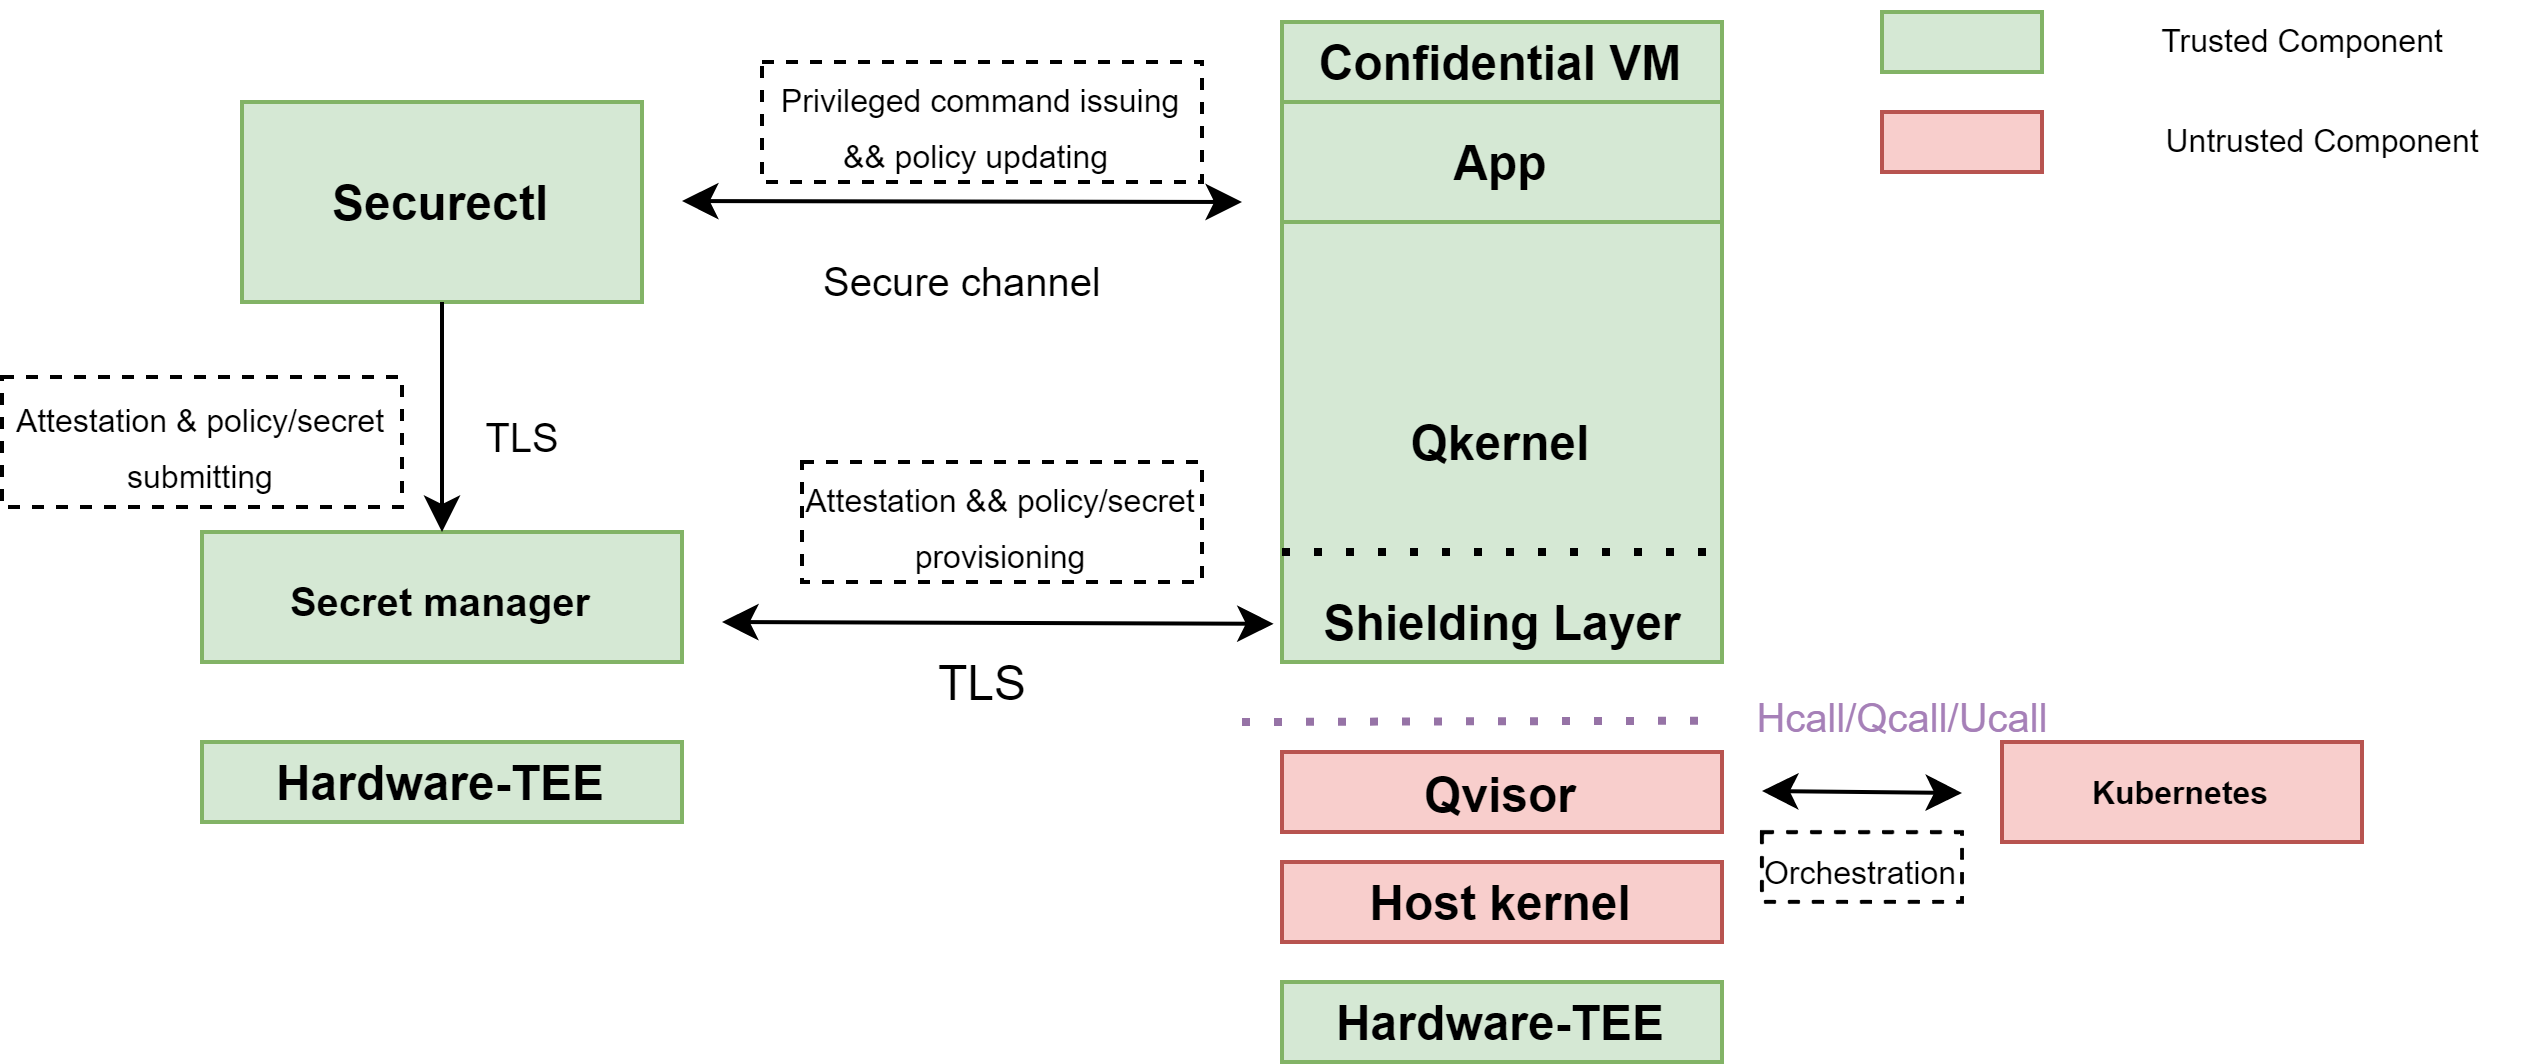
\includegraphics[height=0.3\textheight, width=1\textwidth]{images/genaral_architechture.png}
    \caption[General Architecture]{General Architecture. The green components in the figure are trusted, and the red ones are not.}
    \label{fig:genaral_architechture}
\end{figure}

The overall architecture is depicted in Figure~\ref{fig:genaral_architechture}. It consists of the secret manager, securectl, and a \acrshort{CVM} that runs Qkernel and an application. Notably, a shielding layer is incorporated into the Qkernel to prevent adversaries from exploiting the Hcall, Qcall, and Ucall interfaces to launch attacks on the CVM. As this shielding 
layer is part of the Qkernel, its state is protected by the \acrshort{CVM}. The secret manager manages secrets and operates within a hardware-based TEE on the cloud. securectl operates in the local environment of the application owner. It offers an interface for the application owner to interact with the application and control the shield. Moreover, the application 
owner can utilize securectl to attest the secret manager and then upload the secrets through a secure channel. The secret manager can validate the application startup process against the policy uploaded by the application owner and send the secrets securely to the \acrshort{CVM}. Subsequently, the shield takes charge of secret deployment and ensures the confidentiality 
and integrity of the secrets while \acrshort{CVM} runs.

\todo{use ilastic for securectl}

\section{Quark Attestation and Provisioning Infrastructure}
\label{sec:design_Quark_Attestation_and_Provisioning_Infrastructure}

\begin{figure}[!htb]
    \centering
    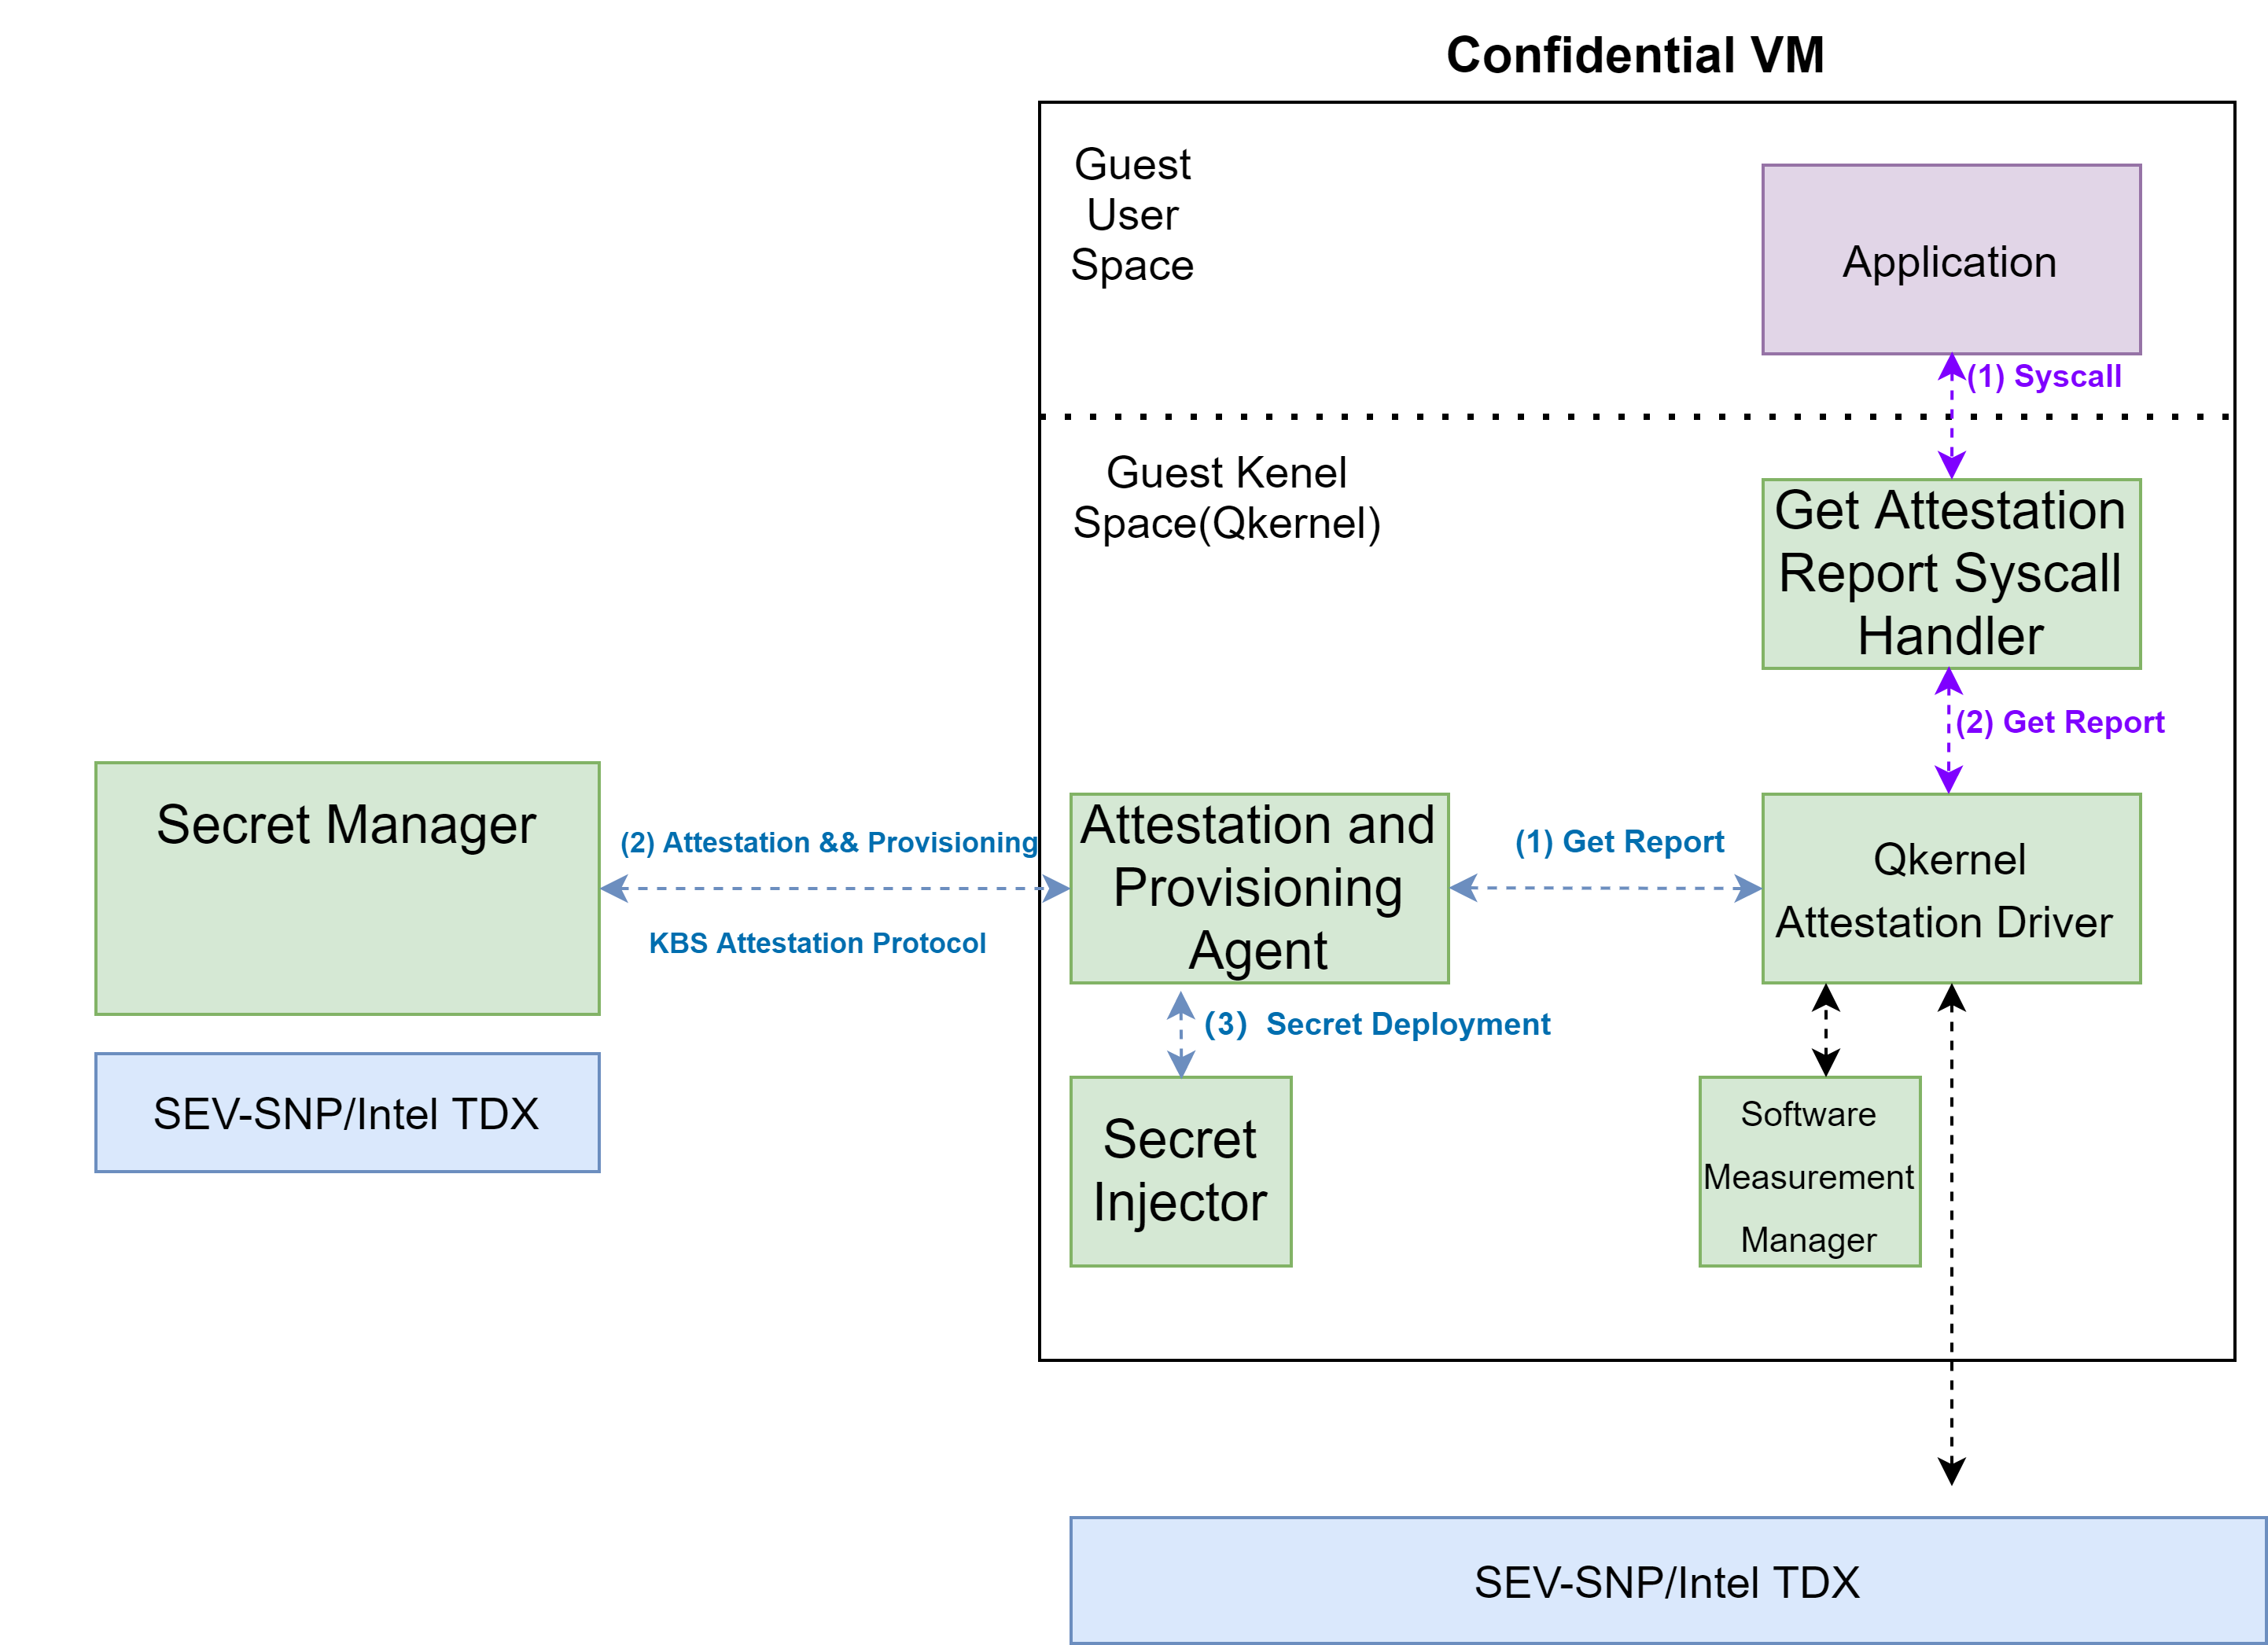
\includegraphics[width=0.8\textwidth]{images/Qkernel_attestation_infrastructurc.png}
    \caption[Quark Attestation and Provisioning Infrastructure]{Quark Attestation and Provisioning Infrastructure}
    \label{fig:Qkernel_attestation_infrastructurc}
\end{figure}


Figure~\ref{fig:Qkernel_attestation_infrastructurc} shows the Quark attestation and provisioning infrastructure. It comprises the secret manager, attestation and provisioning agent, secret injector, attestation report system call handler, Qkernel attestation driver, and software measurement manager. It provides the following services:


This infrastructure enables the secure deployment of secrets during application startup. Before the application process is launched, the remote attestation and provisioning agent uses the KBS attestation protocol~\cite*{kbs_Attestation_protocol} to prove its identity to the secret manager and retrieve secrets, which includes shield policy and application 
secrets (e.g., startup parameters, environment variables, and files). The TEE hardware generates the attestation report required in the protocol with the help of the Qkernel attestation driver. This report contains the shield startup hash. This hash includes measurements made by the software measurement manager on data loaded from the host, such as 
the application binary and the Qkernel configuration file. The secret manager will compare the shield startup hash with a reference value provided by the application owner to ensure that the application and CVM are correctly configured. Once the shield obtains secrets, it utilizes the shield policy to initialize itself. The application’s secrets are 
deployed to the application process by the secret injector. For instance, application startup parameters and environment variables are inserted into the stack of the application process. For file-type secrets, the injector keeps them in virtual machine memory and creates a sub-filesystem using the Qkernel’s virtual filesystem interface. This filesystem is 
mounted in the \textbf{/secret} directory, and applications can access these secrets through this file system. In this way, the secret management and deployment are offloaded from Kubernetes~\cite*{k8s} and Quark shim.


Additionally, the infrastructure allows applications to obtain attestation reports at runtime through the guest system call interface. Note that the system call for getting a report is processed by the attestation report system call handler. For more information, please refer to Section~\ref{sec:runtime_attesation}.

In the following, the secret upload workflow is first explained. Then, the mechanism for the application’s secure deployment and runtime attestation are discussed. For specific implementations of each module, please refer to Section~\ref{sec:impl_attestation_infr}.



\subsection{Secret Uploading}
\label{sec:design_Secret_Uploading}
\begin{figure}[!htb]
    \centering
    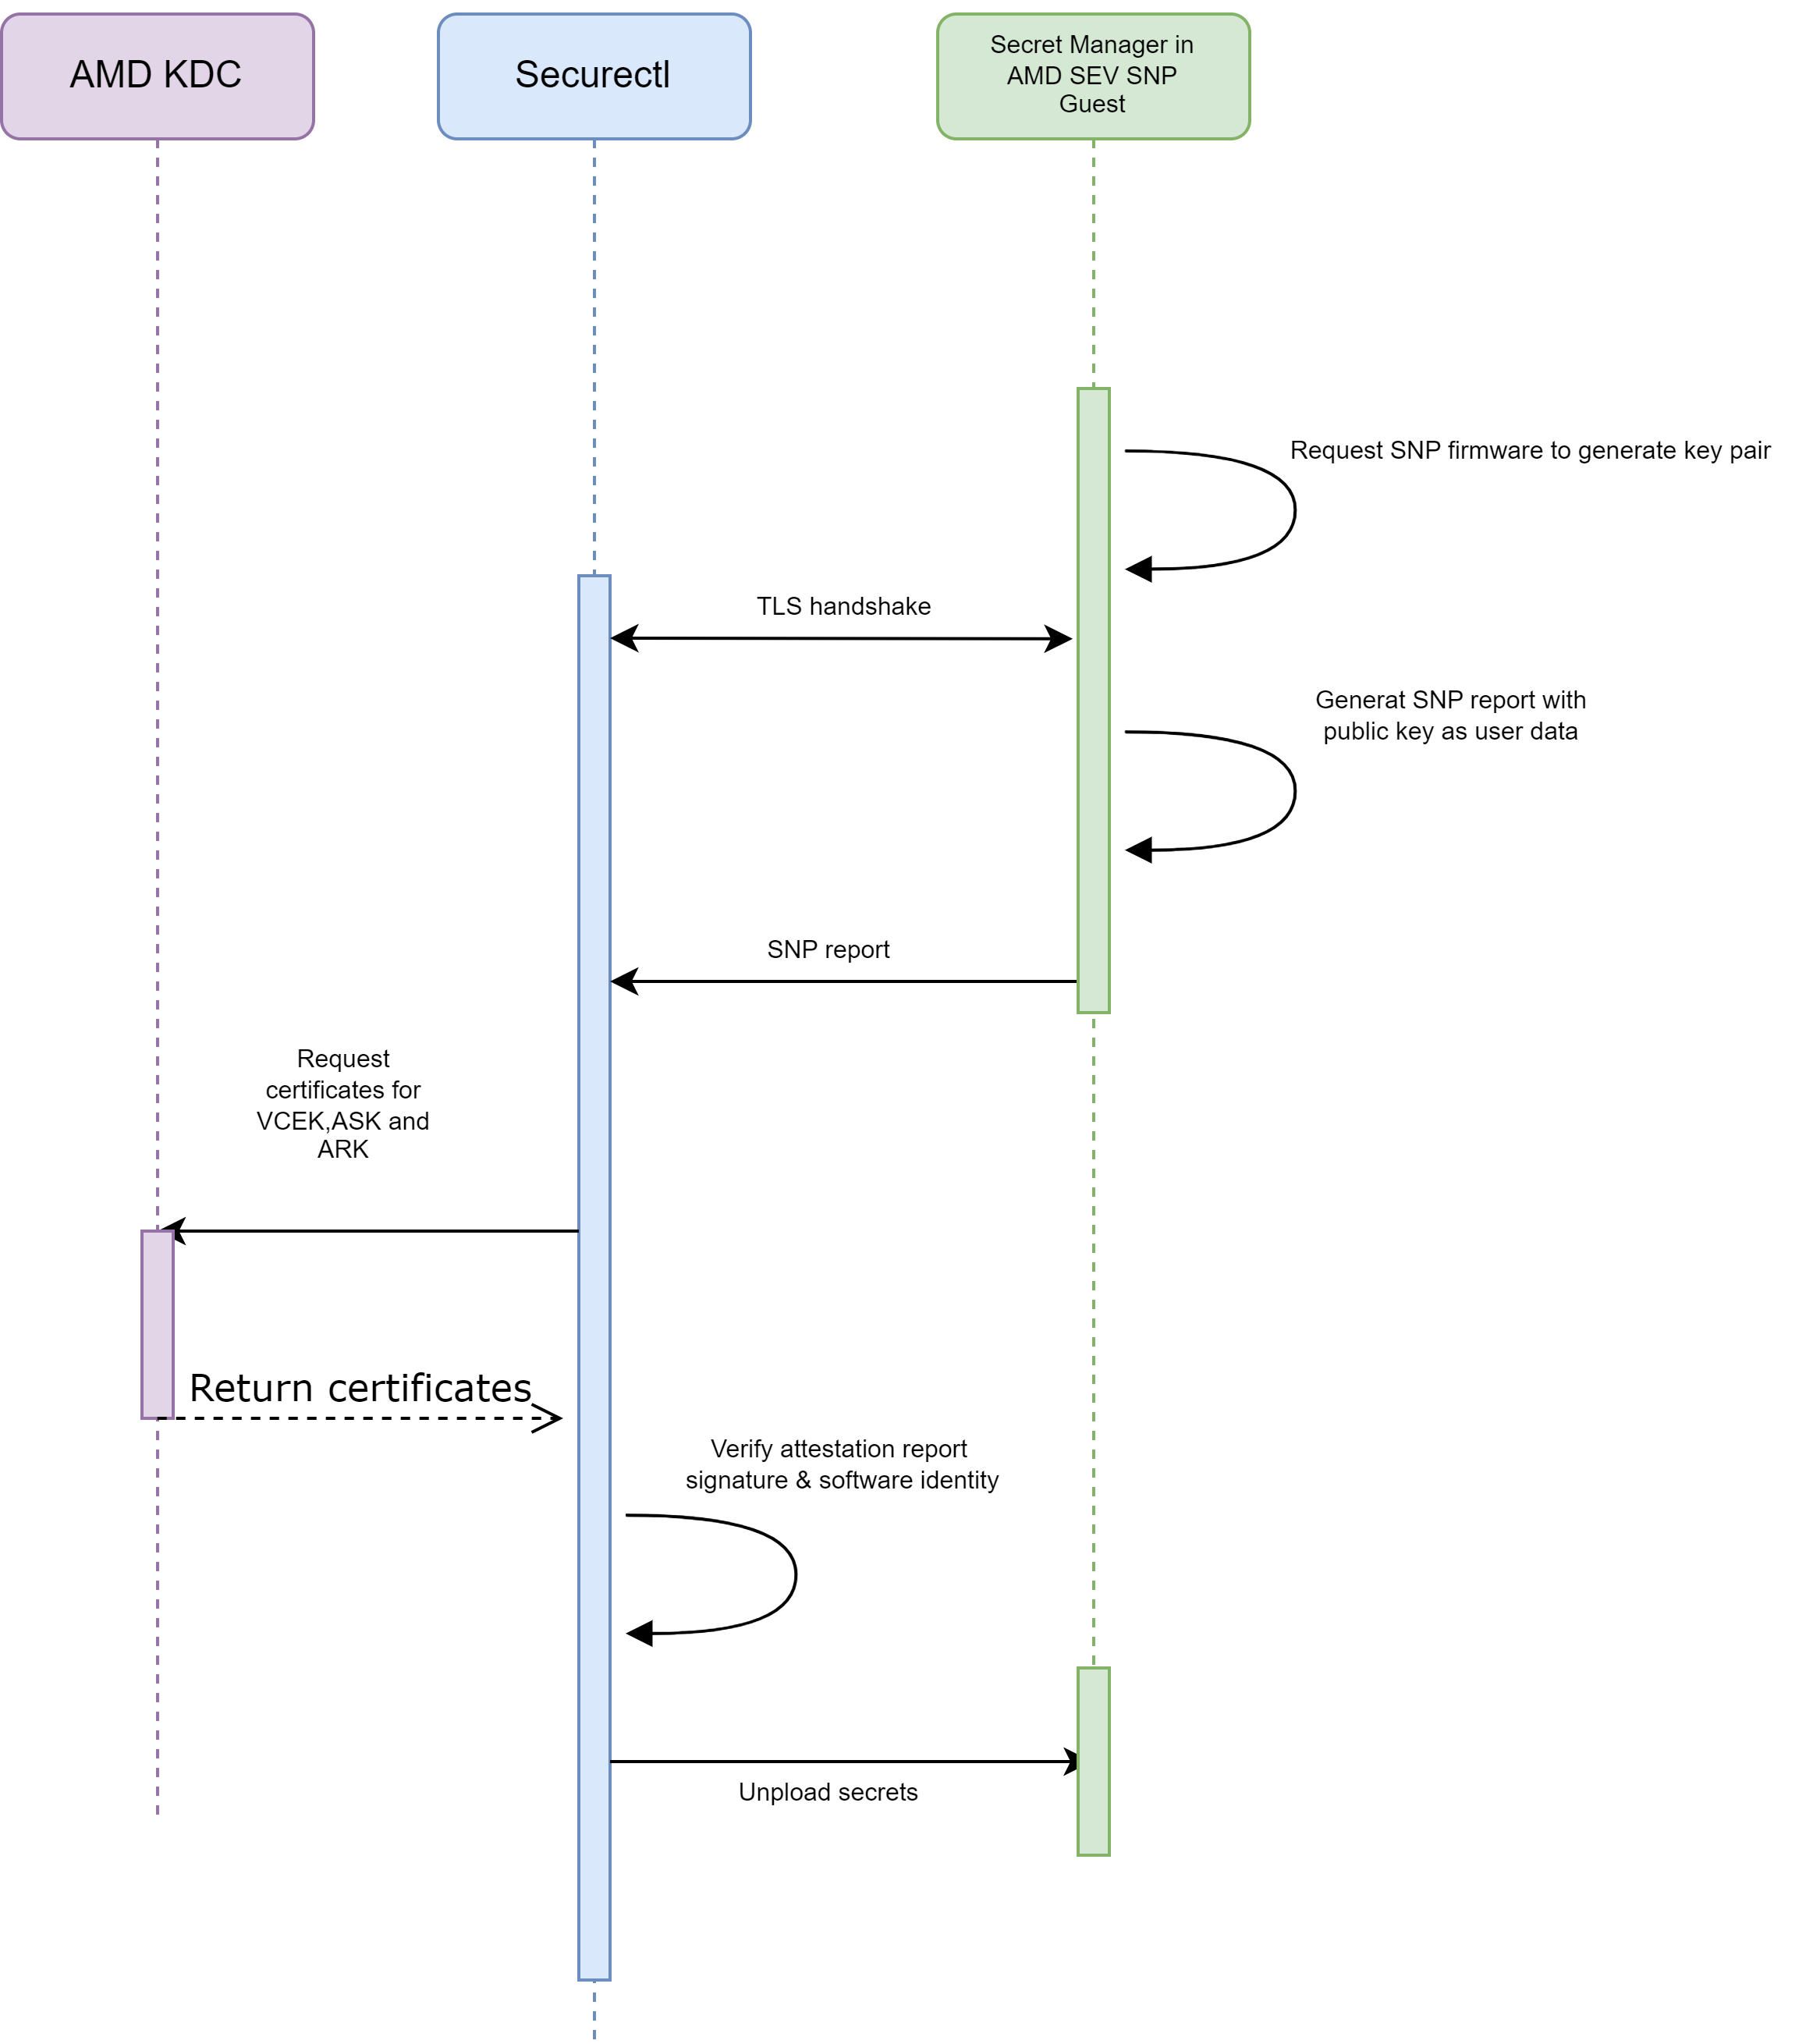
\includegraphics[height=0.4\textheight]{images/upload_secret.png}
    \caption[Secret Uploading Workflow]{Secret Uploading Workflow.}
    \label{fig:upload_secret}
\end{figure}

The process of uploading secrets to the secret manager requires two steps to be taken by the application owner. Firstly, the application owner must validate the secret manager's state using remote attestation. Secondly, a secure channel must be established for secret uploading. This process is illustrated in Figure~\ref{fig:upload_secret}. 
Note that the thesis assumes the secret manager runs in the AMD SEV-SNP~\ref{fig:upload_secret}. Initially, the secret manager generates an RSA key pair for the TLS~\cite*{tls_record_size} connection and stores the private key in its memory. This key can be regarded as an identifier for the secure channel. To bind the secret manager to the identifier of the secure channel, the hash of the RSA public key is added to the attestation report of the secret manager. 
Upon receiving the report, the application owner requests a certificate chain from the AMD KDC~\cite*{snp_kdc}. The certificate chain is then used to verify the signature of the report. Then using the information in the report, the application owner can ensure that the secret manager is genuine and that the hash of the public key used to establish the TLS matches the hash of the public key 
in the report. By fulfilling these steps, the application owner can determine that the entity on the other side of the secure channel is an expected secret manager. Thus, the channel can safely be leveraged for secrets uploading.


\subsection{Secure Application Deployment}
\label{sec:secure_application_deployment}
\begin{figure}[!htb]
    \centering
    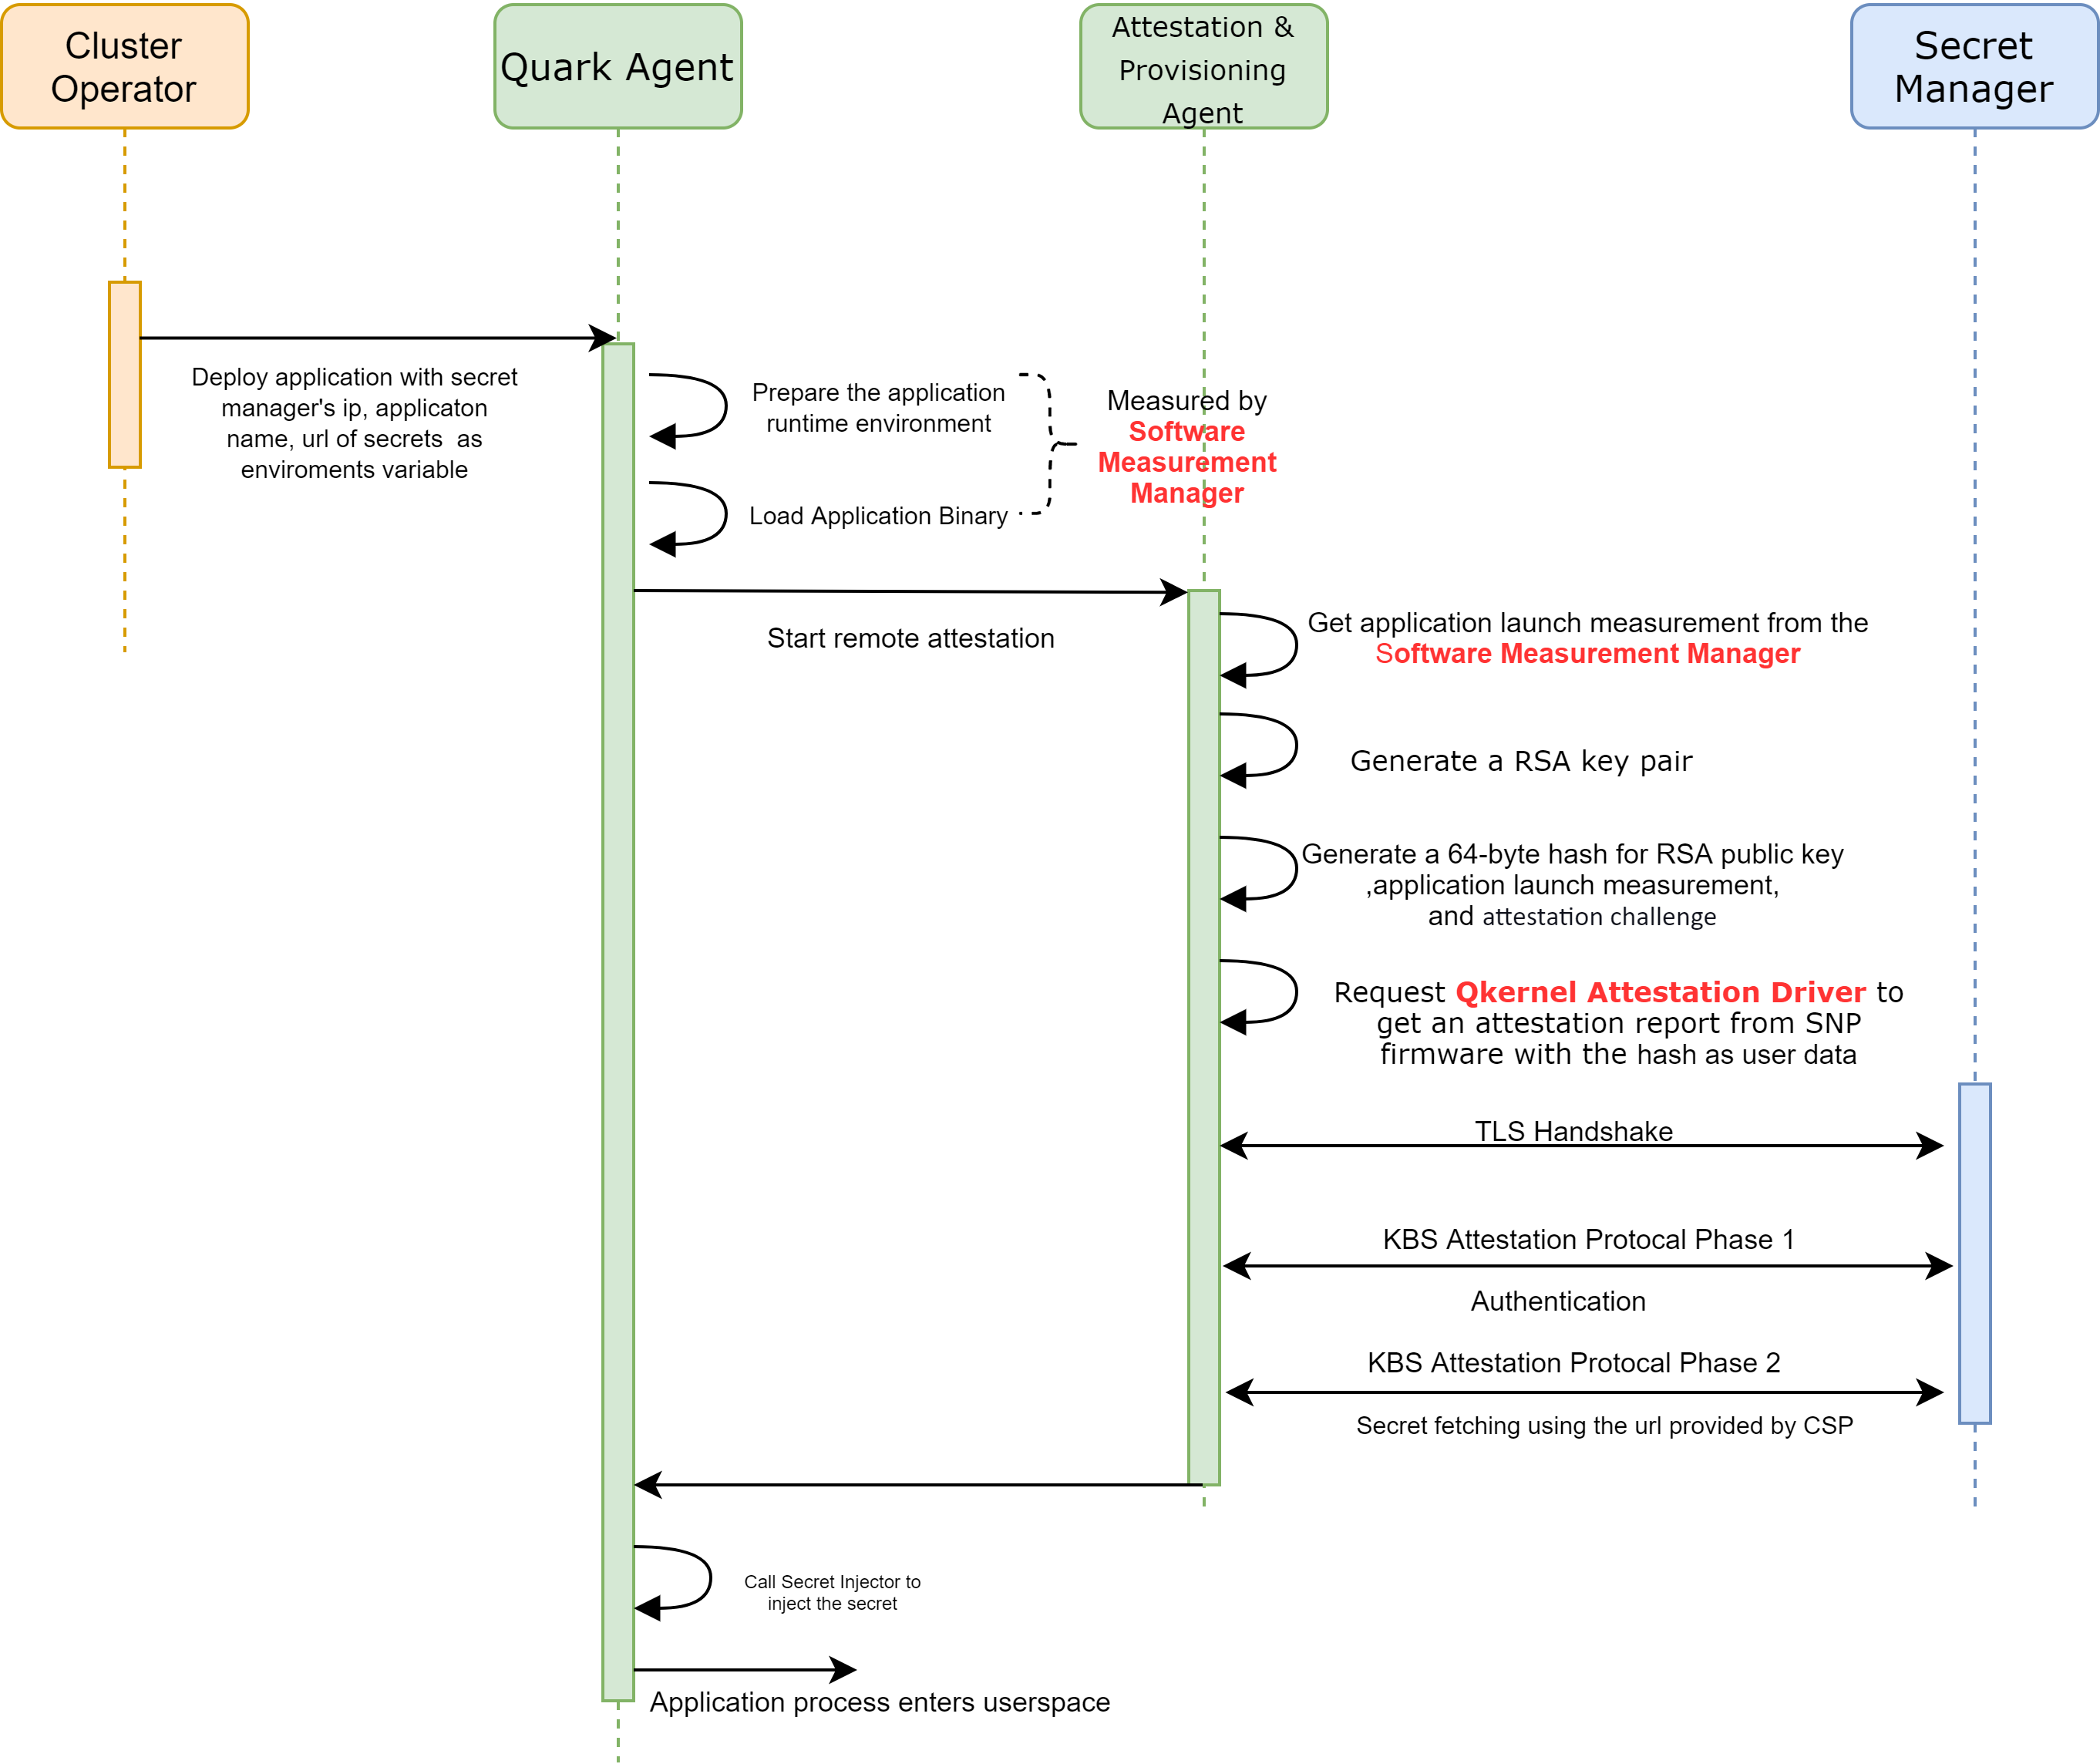
\includegraphics[height=0.5\textheight]{images/attestation_provisioning.png}
    \caption[Secure Application Deployment Workflow]{Secure Application Deployment. The green components are running in the \acrshort{CVM}. The cluster operator is not trusted. The secret manager is responsible for managing the secrets, attesting enclaves, and provisioning the secrets.}
    \label{fig:attestation_provisioning}
\end{figure}
Secure application deployment aims to ensure the confidentiality and integrity of the application’s secrets and the shield’s policy. As such, a new secret deployment mechanism is proposed in Figure~\ref{fig:attestation_provisioning}.

The cluster operator still uses a YAML configuration file to deploy applications but without including any secrets. Instead, application secrets and the shield policy are uploaded to the secret manager. The cluster operator only needs to pass the IP address of the secret manager, secrets’ URLs, and the application binary’s name as the environment variable 
to the \acrshort{CVM}. 

Upon receiving an application creation request, the quark agent located in the \acrshort{CVM} creates the application process according to the process configuration. Remote attestation and secret provisioning occur after the CVM loads the application binary. This ensures that the secret manager can verify the integrity of the loaded application binary. 
However, before creating the application process, the \acrshort{CVM} may need to load and execute multiple binaries to set up the application’s runtime environment. Therefore, the \acrshort{CVM} will use the name of the application binary in the YAML file to determine if the application binary is loaded. Once loaded, the quark agent will trigger remote attestation 
and provisioning agent.

The agent first requests the Qkernel attestation driver to generate an attestation report. Depending on the type of TEE, the driver will generate different attestation reports. Assuming the CVM runs in AMD SEV-SNP~\cite*{SEV_SNP_white_book}, the driver will request the SEV-SNP firmware to create a SEV-SNP report. The agent will then connect to the secret manager 
using the IP address in the YAML file and establish a TLS connection. Once the TLS handshake is completed, the agent will complete remote attestation and provisioning according to the KBS attestation protocol~\cite*{kbs_Attestation_protocol}. Specifically, in the authentication phase, it uses the attestation report generated by the Qkernel attestation driver to 
prove its identity to the secret manager. In the second phase, it will use the URLs in the YAML file to construct HTTP GET requests to retrieve the secrets from the secret manager. For a detailed explanation of the KBS protocol, please refer to Section~\ref{sec:kbs}.

The format of the SEV-SNP report is shown in Figure~\ref*{fig:attestation_report_format}. The report is protected with the~\acrshort{VCEK} signature and contains SEV-SNP firmware's measurements for the VM boot process, tamper-resistant 64-byte user-defined data, host data, and others. 


\begin{figure}[!htb]
    \centering
    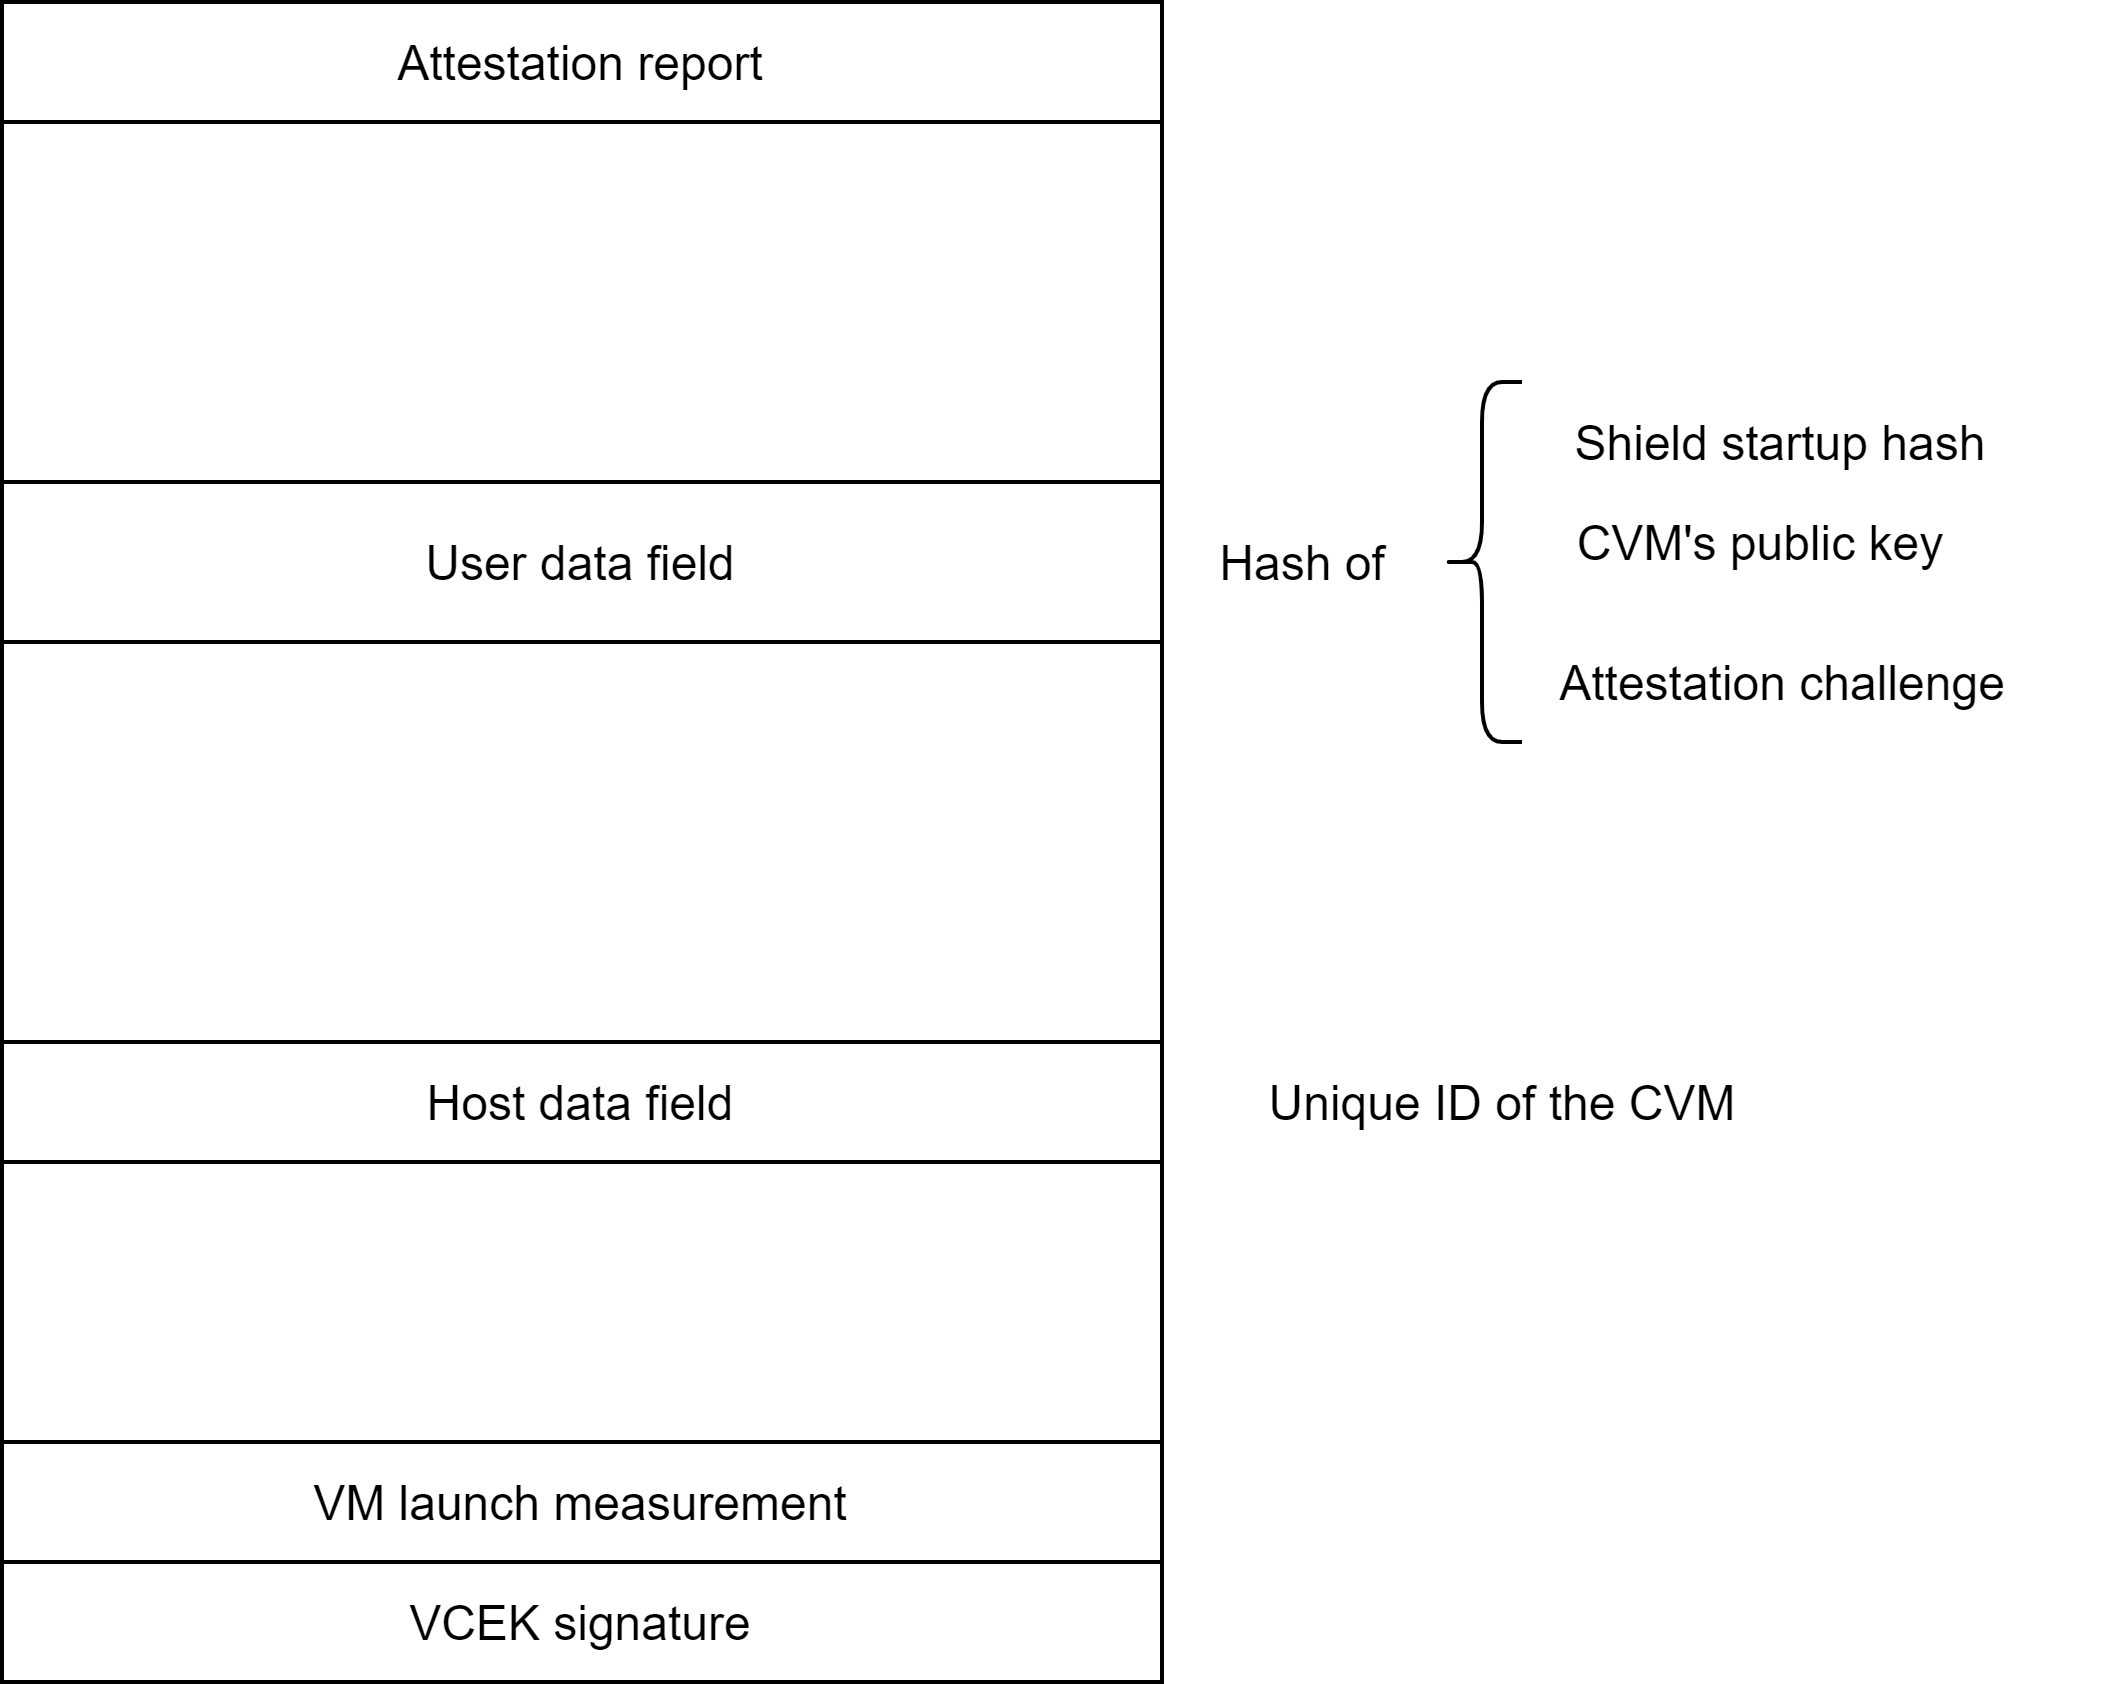
\includegraphics[height=0.3\textheight]{images/attestation_report_format.png}
    \caption[SEV-SNP attestation report]{SEV-SNP attestation report~\cite*{snp_firmware}}
    \label{fig:attestation_report_format}
\end{figure}

The secret manager can verify the report's signature using the certificate chain required by AMD KDC~\cite*{snp_kdc}. By checking the measurements of the virtual machine boot process, the secret manager can confirm that the CVM is using the correct Qkernel binary because the Qkernel is loaded into the CMV memory by Qvisor using 
\todo{new font for the defination} SNP\_LAUNCH\_UPDATE~\cite*{snp_firmware} before VM boot. Notably, the code of the shielding layer is part of the Qkernel binary.

The user-defined data in the report is a hash of the shield startup hash and metadata required by the KBS protocol~\cite*{kbs_Attestation_protocol}. These metadata include a RAS public key representing the identity of the \acrshort{CVM} and an attestation challenge assigned by the secret manager. An explanation of these metadata can be found in Section~\ref{sec:kbs}. The software measurement 
manager creates the shield startup hash and incorporates all the sensitive data that the \acrshort{CVM} loads from the host after the \acrshort{CVM} starts. This includes Qkernel command line argument (i.e., Qkernel configuration file~\cite*{quark_conf_file}), binaries, shared libraries, and the public key of the secret manager. By comparing the shield startup hash
to a reference hash provided by the application owner, the secret manager can ensure that the \acrshort{CVM} is configured correctly and that only legitimate binaries are loaded. The secret manager's public key is used for application runtime attestation discussed in Section~\ref{sec:runtime_attesation}.

In order to prevent an attacker from hijacking the secret manager's address and impersonating the secret manager, the KBS attestation protocol~\cite*{kbs_Attestation_protocol} requires that the CVM uses the secret manager's public key to authenticate the secret manager during the TLS handshake. Currently, Kubernetes~\cite*{k8s} mounts the public key as a file on 
the application's rootfs. The \acrshort{CVM} reads the public key into the guest memory and uses it to set up the TLS connection to the secret manager. When an attacker provides the public key of a fake secret manager to the \acrshort{CVM}, the TLS handshake fails due to a mismatch between the public key and the certificate of the real secret manager. In other words, the 
\acrshort{CVM} can only establish a connection with the fake secret manager.



\label{eq:1}The KBS attestation protocol~\cite*{kbs_Attestation_protocol} needs improvement. Since all \acrshort{CVM} uses a standard Qkernel binary and applications are created from classic images, the attestation evidence cannot uniquely identify an enclave. Instead, the evidence only certifies that the attester is an enclave running in a TEE with the correctly 
loaded guest kernel and application. When a secret manager manages the secrets of multiple stakeholders, a \acrshort{CVM} belonging to one stakeholder could steal the secrets of another. To address this issue, the application owner should assign a unique ID to each CVM. This ID should be added to the host data field of the attestation report by Qvisor before 
the \acrshort{CVM} starts. This field is immutable after launching the \acrshort{CVM}, so the ID is bound to the \acrshort{CVM}'s attestation evidence. When the secret manager receives a \acrshort{CVM}'s attestation report, it can use this ID to determine the \acrshort{CVM}'s identity. In the authentication phase of the KBS attestation 
protocol~\cite*{kbs_Attestation_protocol}, the secret manager should bind not only the authentication result but also the \acrshort{CVM}'s ID to the cookie identifier. This way, the secret manager can map the cookie identifier in the attester's resource request message to its attestation result and the \acrshort{CVM}'s ID. As such, the secret manager can use the 
ID and the secret owner's policy to determine whether to grant access to a particular secret to the \acrshort{CVM}. The attester's resource request URL should have the following format: \emph{<repository>/<type>/<tag>}, where \emph{<repository>} is similar to the concept of container image repository,\emph{<type>} is used to distinguish between different resource 
types, and \emph{<tag>} is used to distinguish different versions of a resource. The secret manager should assign each user a unique repository and let them specify which \acrshort{CVM} with which IDs can access this repository. To this end, the cross-leakage of secrets between different stakeholders can be effectively avoided. 


Note that some of the above features are not implemented. Section~\ref{subsec:Limitations} summarizes the limitations of secure application deployment.

\subsection{Application Runtime Attestation Service}
\label{sec:runtime_attesation}

An application may need to attest itself to a remote party at runtime. Quark attestation and provisioning infrastructure enable applications to obtain attestation reports through the guest system call interface. Depending on the application's needs, one of three report formats can be 
obtained: an attestation report generated by the \acrshort{TEE} hardware and two software attestation reports created by the shielding layer. The latter contains:

\begin{itemize}
    \item Shield startup hash.
    \item \acrshort{CVM} ID.
    \item Signature.
    \item Sixty-four bytes of application-specified data.
\end{itemize}

The application can sign the software report with a key issued by the secret manager or by a key it provided. The secret manager's key is sent to the \acrshort{CVM} along with the application's secret during the secure application deployment. Software reports offer additional possibilities 
for how the application proves its identity to the remote party. In other words, the remote party can verify the report without the assistance of the CPU vendor. Upon verification of the report, the remote party can ensure that the application is as expected by using the shield startup 
hash. Besides, application-defined data in a software report is tamper-proof, similar to user data in SEV-SNP reports. As previously discussed, the \acrshort{CVM} ID guarantees that the remote party can determine the application's identity, which prevents secret cross-leakage. Section~\ref{sec:secure_application_deployment} has already discussed the major 
benefits of shield startup hash. Additionally, it includes the measurement of the secret manager's public key. Therefore, the remote party can be sure that the \acrshort{CVM} acquired the secrets from the genuine secret manager during application startup and 
correctly initialized the shielding layer. In other words, if the shielding layer is initialized with a compromised policy acquired from a fake secret manager, it can no longer guarantee that the secrets provisioned by the remote party won't be leaked.


\section{\acrshort{CVM} Runtime Measurement}
\label{sec:Enclave_Runtime_Measurement}
\begin{figure}[!htb]
    \centering
    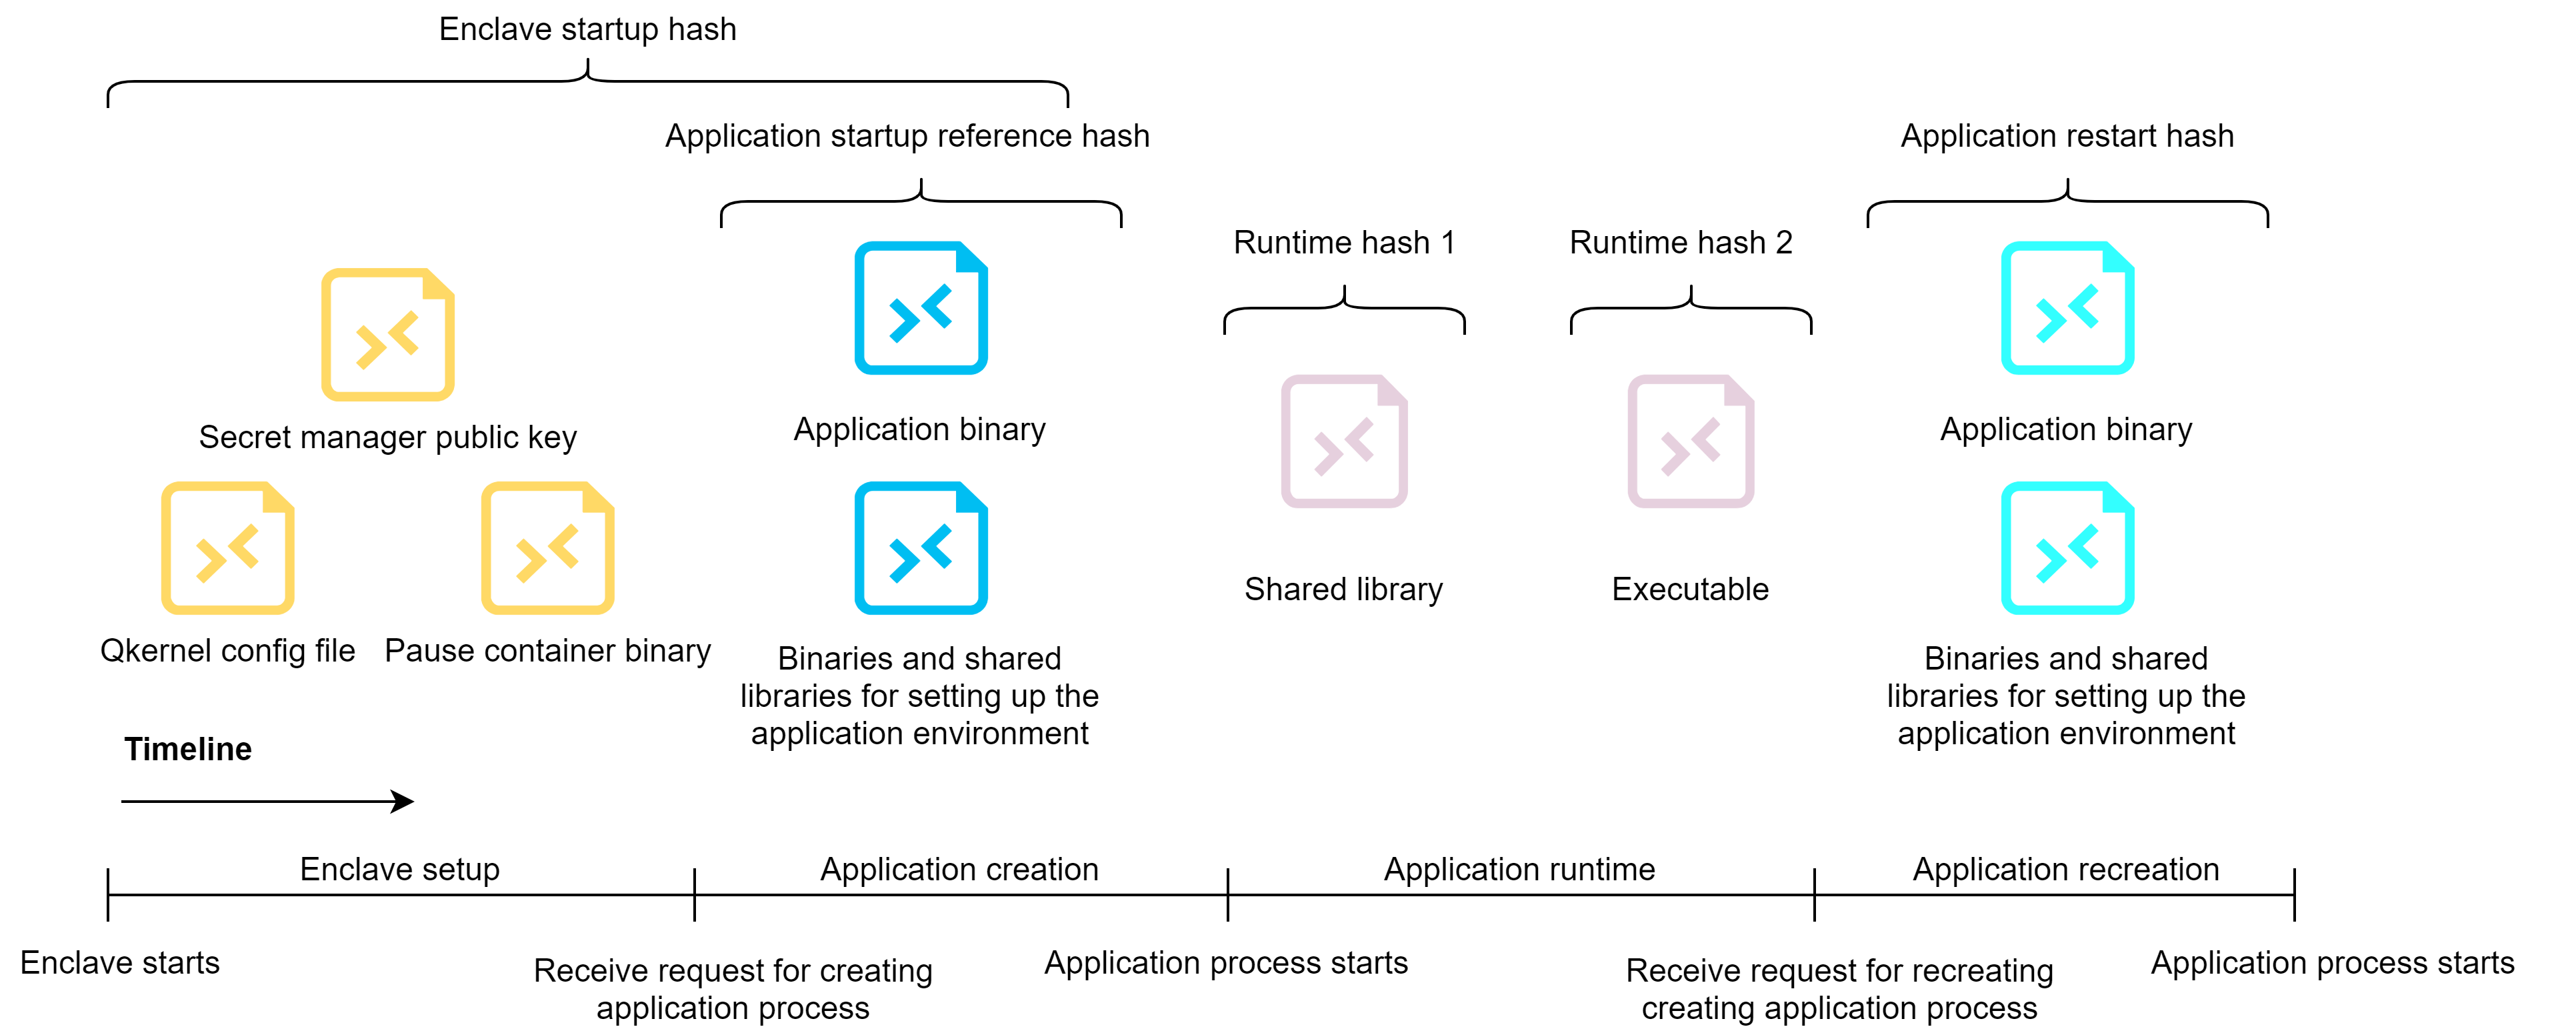
\includegraphics[width=1\textwidth]{images/soft_ware_manager_meausrment.png}
    \caption[\acrshort{CVM} runtime measurement]{\acrshort{CVM} runtime measurement}
    \label{fig:soft_ware_manager_meausrment}
\end{figure}

Enclave runtime measurements are crucial due to the security analysis findings discussed in Chapter~\ref{sec:security_analyse}. However, the AMD SEV SVP does not support enclave runtime measurements~\cite*{snp_firmware}, and the INTEL TDX only allocates four registers for this purpose~\cite*{Intel_tdx_whitepaper}. Consequently, we provide a software measurement 
manager in the shielding layer to measure the data loaded from the host while the enclave is running. As shown in Figure~\ref{fig:soft_ware_manager_meausrment}., The software measurement manager provides the following important hashes:

\textbf{Enclave startup hash.} This value refers to the measures of host-loaded data until the application process starts. This includes the secret manager's key, the Qkernel's configuration file, the application's binary, and multiple binaries and shared libraries loaded to set up the application environment. Notably, since each Pod uses a pause container to hold the 
sandbox's metadata, the enclave startup hash also contains a measurement of the binaries and shared libraries loaded when the pause container was created. The attestation and provisioning agent include this hash in the attestation report, which is conveyed to the secret manager. The secret manager compares the measurement to the reference value provided 
by the enclave owner to ensure the enclave is properly configured. This hash effectively solves the problems~\ref{vulnerabilities:1},~\ref{vulnerabilities:7},~\ref{vulnerabilities:11} identified in Chapter~\ref{sec:security_analyse}.


\textbf{Application startup reference hash.} As shown in the figure, this value records the measure of all binaries and shared libraries loaded during the application's first startup. This measurement is a subset of the enclave's startup measurements and is stored in the enclave's memory. It will be used as a reference value for the application restart hash to ensure the 
the integrity of the binary and shared libraries load during the restart. 

\textbf{Runtime hash.} The runtime hash represents a measurement of an executable or shared library loaded in the application runtime. Unlike the enclave startup hash, which is forwarded to the secret manager, the runtime hash is verified by the software measurement manager. The shielding layer's policy holds reference hashes, as shown in Figure~\ref{fig:measurement}. In this case, 
the software measurement manager measures a binary and compares the result with the reference value from the policy. If the two values differ, the enclave will panic. This ensures the correct shared library or executable is loaded during application runtime.
\begin{figure}[!htb]
    \centering
    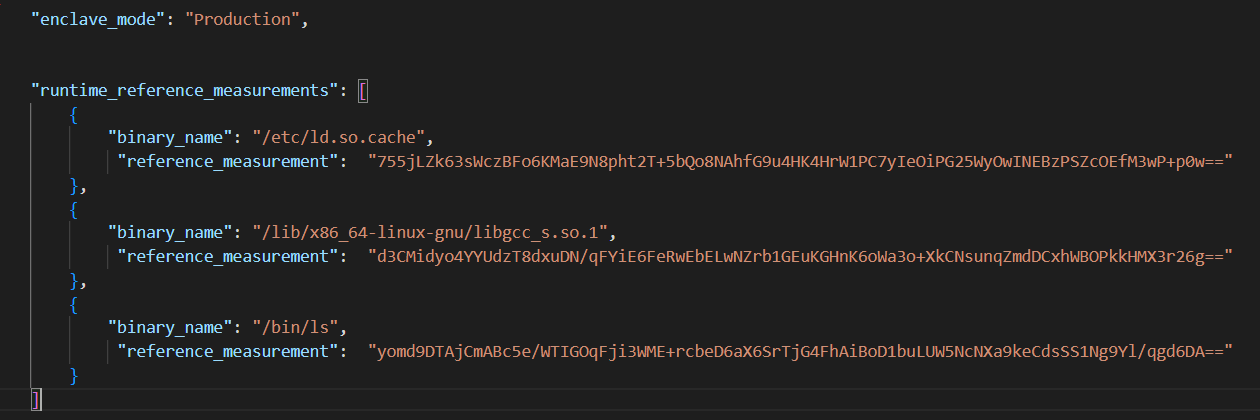
\includegraphics[width=0.8\textwidth]{images/measurement.png}
    \caption[Reference value in shielding layer's policy for runtime hashes]{Reference value in shielding layer's policy for runtime hashes}
    \label{fig:measurement}
\end{figure}

\textbf{Application restart hash.} The software measurement manager measures the binaries and shared libraries when the application crashes and restarts. The resulting application restart hash will be compared with the application startup reference hash before launching the application process. If the two do not match, the enclave panics. In this way, the enclave 
ensures that the host data loaded at restart is the same as the data from the first application startup. The application startup reference hash is a subset of the enclave's startup hash, checked by the secret manager. Thus comparing the two hashes ensures the integrity of the binaries and shared libraries loaded at application restart. 

Regarding obtaining the reference values for enclave startup hash and runtime hashes, we implemented an enclave mode called Development. When running in this mode, the enclave will print these hashes to the Qkernel log on the host. The enclave owner should run the enclave in a trusted environment to obtain these reference values.

\section{New Pattern for EXEC Requests}
\label{sec:design_EXEC_Requests}
\begin{figure}[!htb]
    \centering
    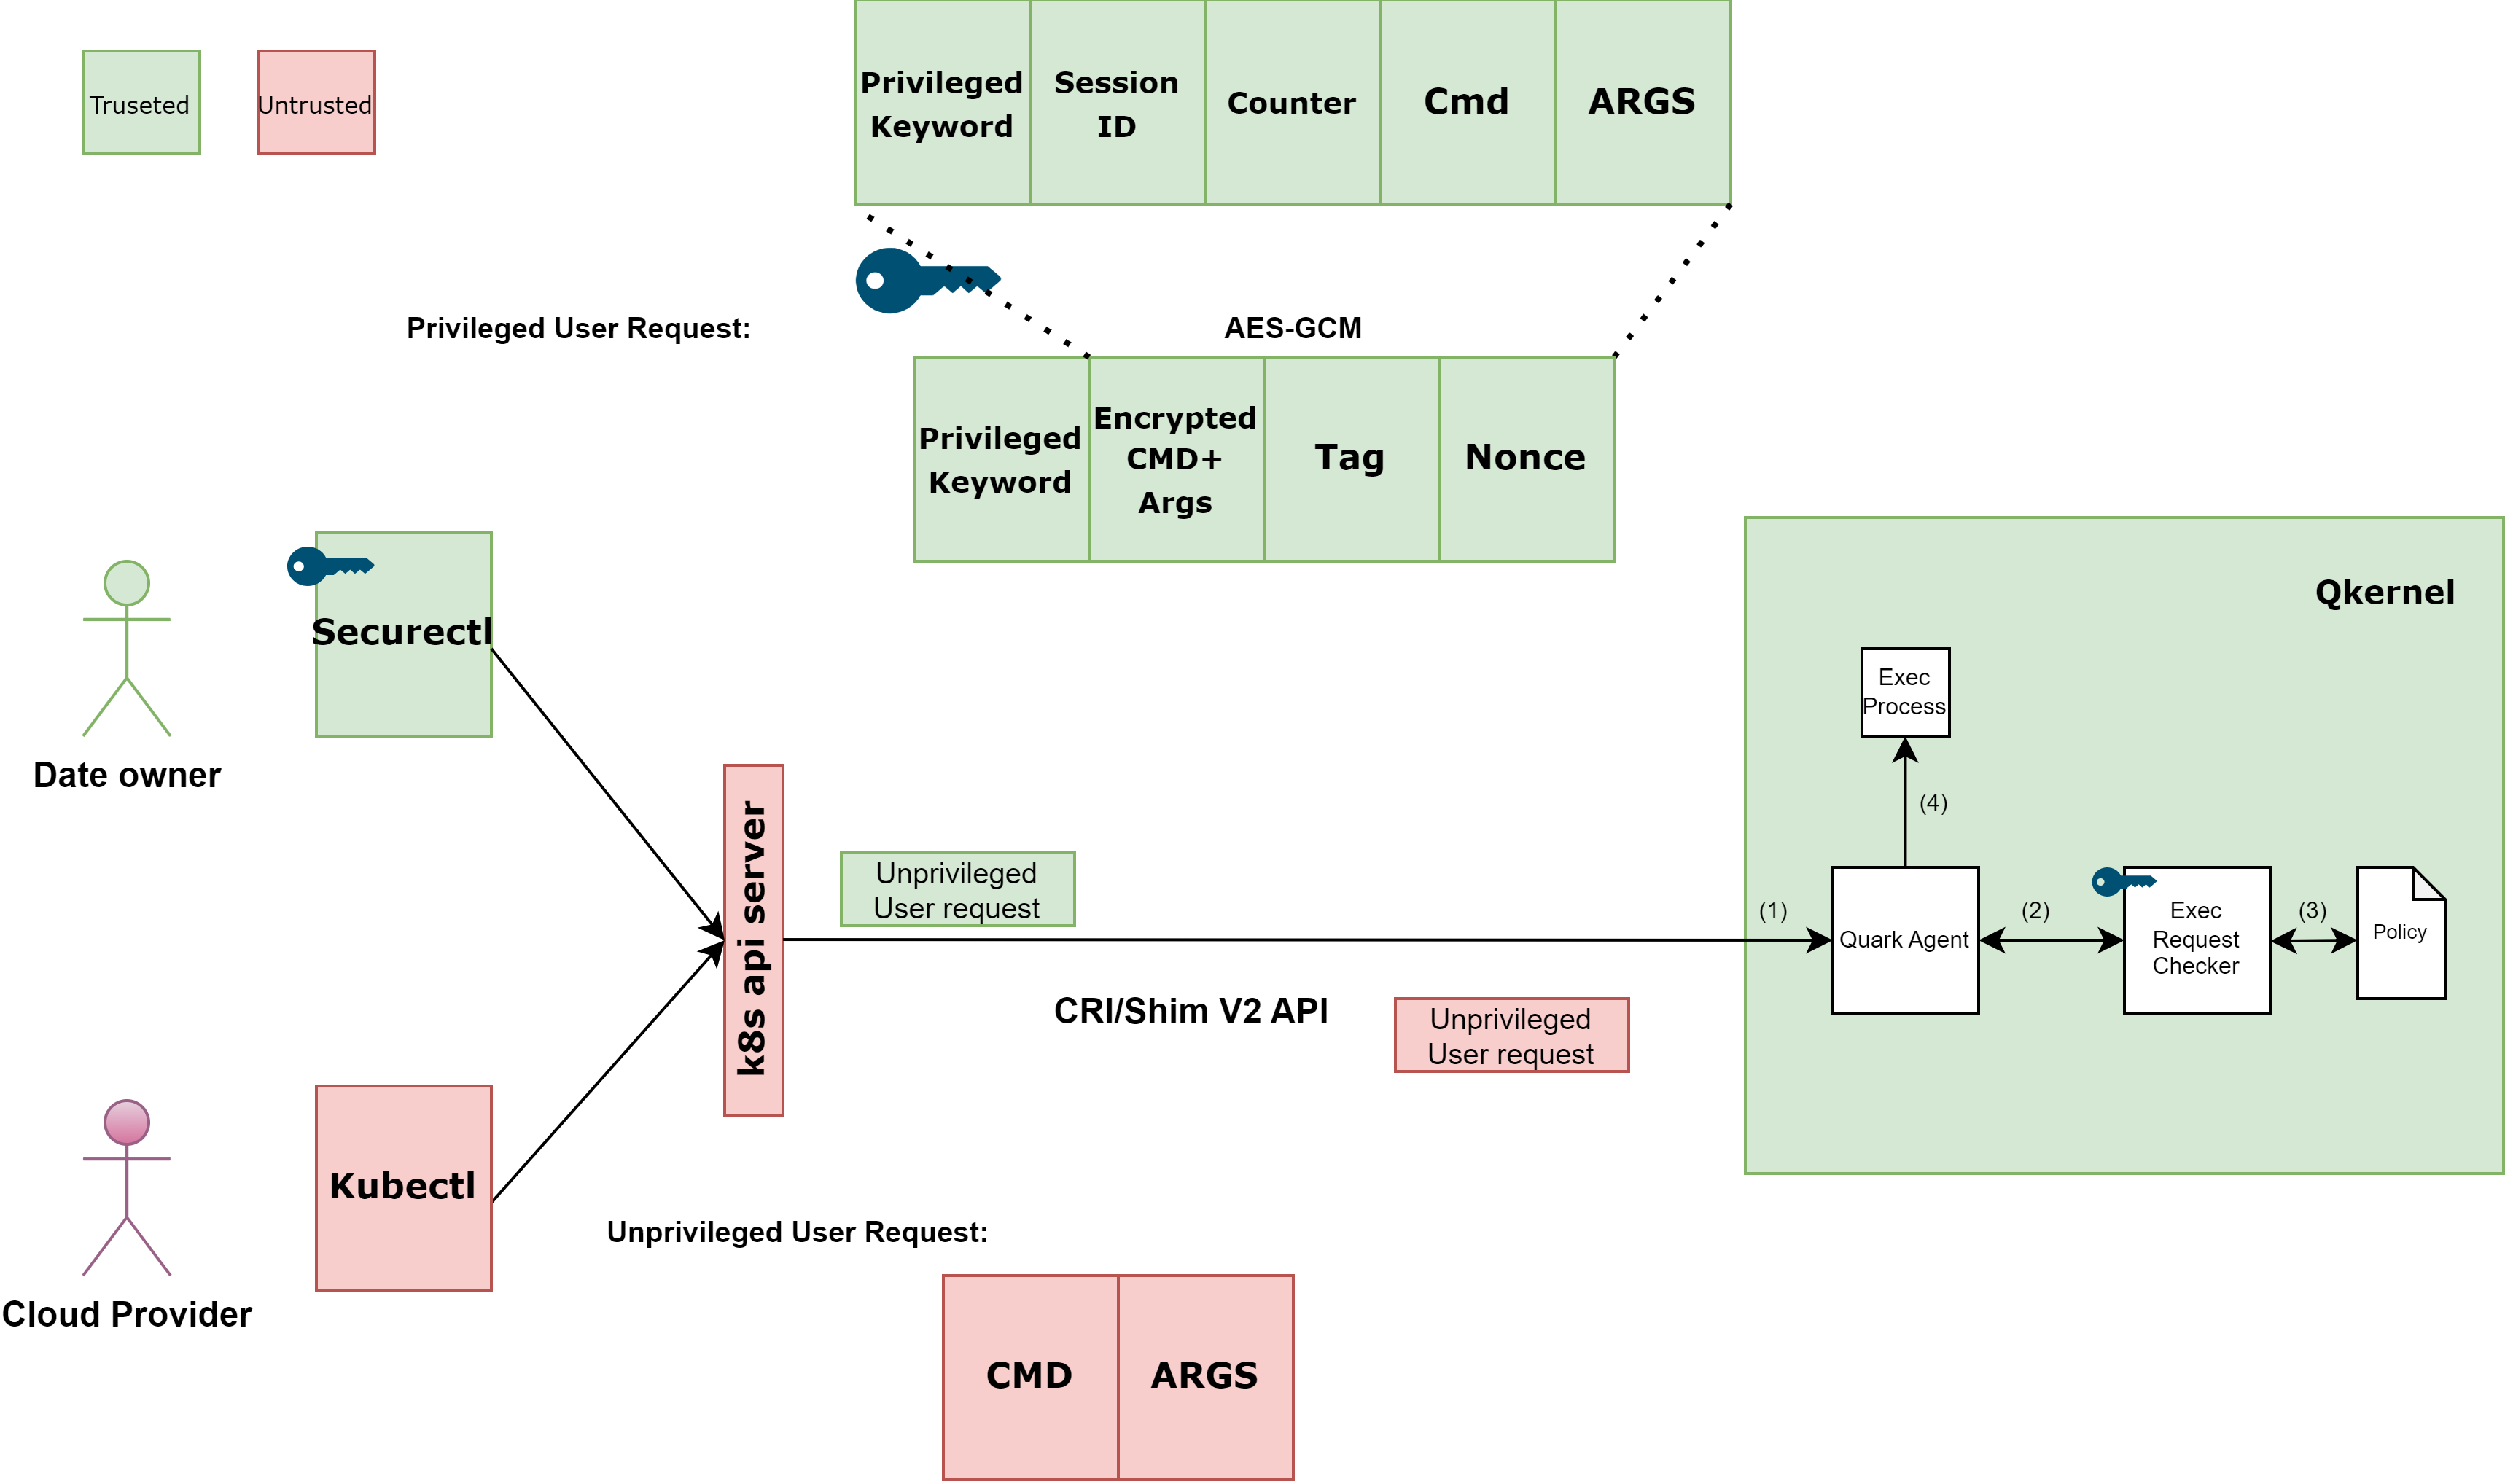
\includegraphics[width=0.8\textwidth]{images/new_pattern_of_exec.png}
    \caption[New pattern for EXEC requests]{New pattern for EXEC requests}
    \label{fig:new_pattern_of_exec}
\end{figure}

We propose a new pattern for EXEC requests to address issues ~\ref{vulnerabilities:4} and ~\ref{vulnerabilities:6} identified in the security analysis. As illustrated in Figure~\ref{fig:new_pattern_of_exec}, The design divides EXEC requests into two categories, namely privileged and unprivileged EXEC requests. 
Privileged EXEC requests are issued by privileged users (i.e., enclave owners), while untrusted entities issue unprivileged requests. An untrusted entity here refers to someone other than the enclave owner. Privileged and non-privileged users send privileged or non-privileged requests to the enclave using securectl or kubectl, respectively. Both requests
are redirected to the enclave through the Kubernetes~\cite*{k8s}. Upon receiving an EXEC request, the Quark agent forwards it to the EXEC request checker. According to the enclave policy, the EXEC request checker will authenticate and access control the request. The Quark agent will decide whether to create the 
EXEC process based on the result returned by the EXEC request checker.

\begin{figure}[!htb] 
    \begin{subfigure}[b]{0.3\linewidth}
      \centering
      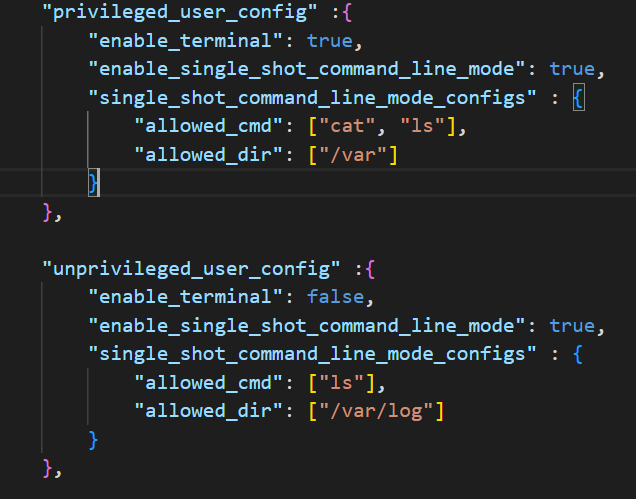
\includegraphics[width=0.9\linewidth]{images/exec_policy.png} 
      \caption{Policy for EXEC requests} 
      \label{fig:exec_policy} 
      \vspace{4ex}
    \end{subfigure}%% 
    \begin{subfigure}[b]{0.6\linewidth}
      \centering
      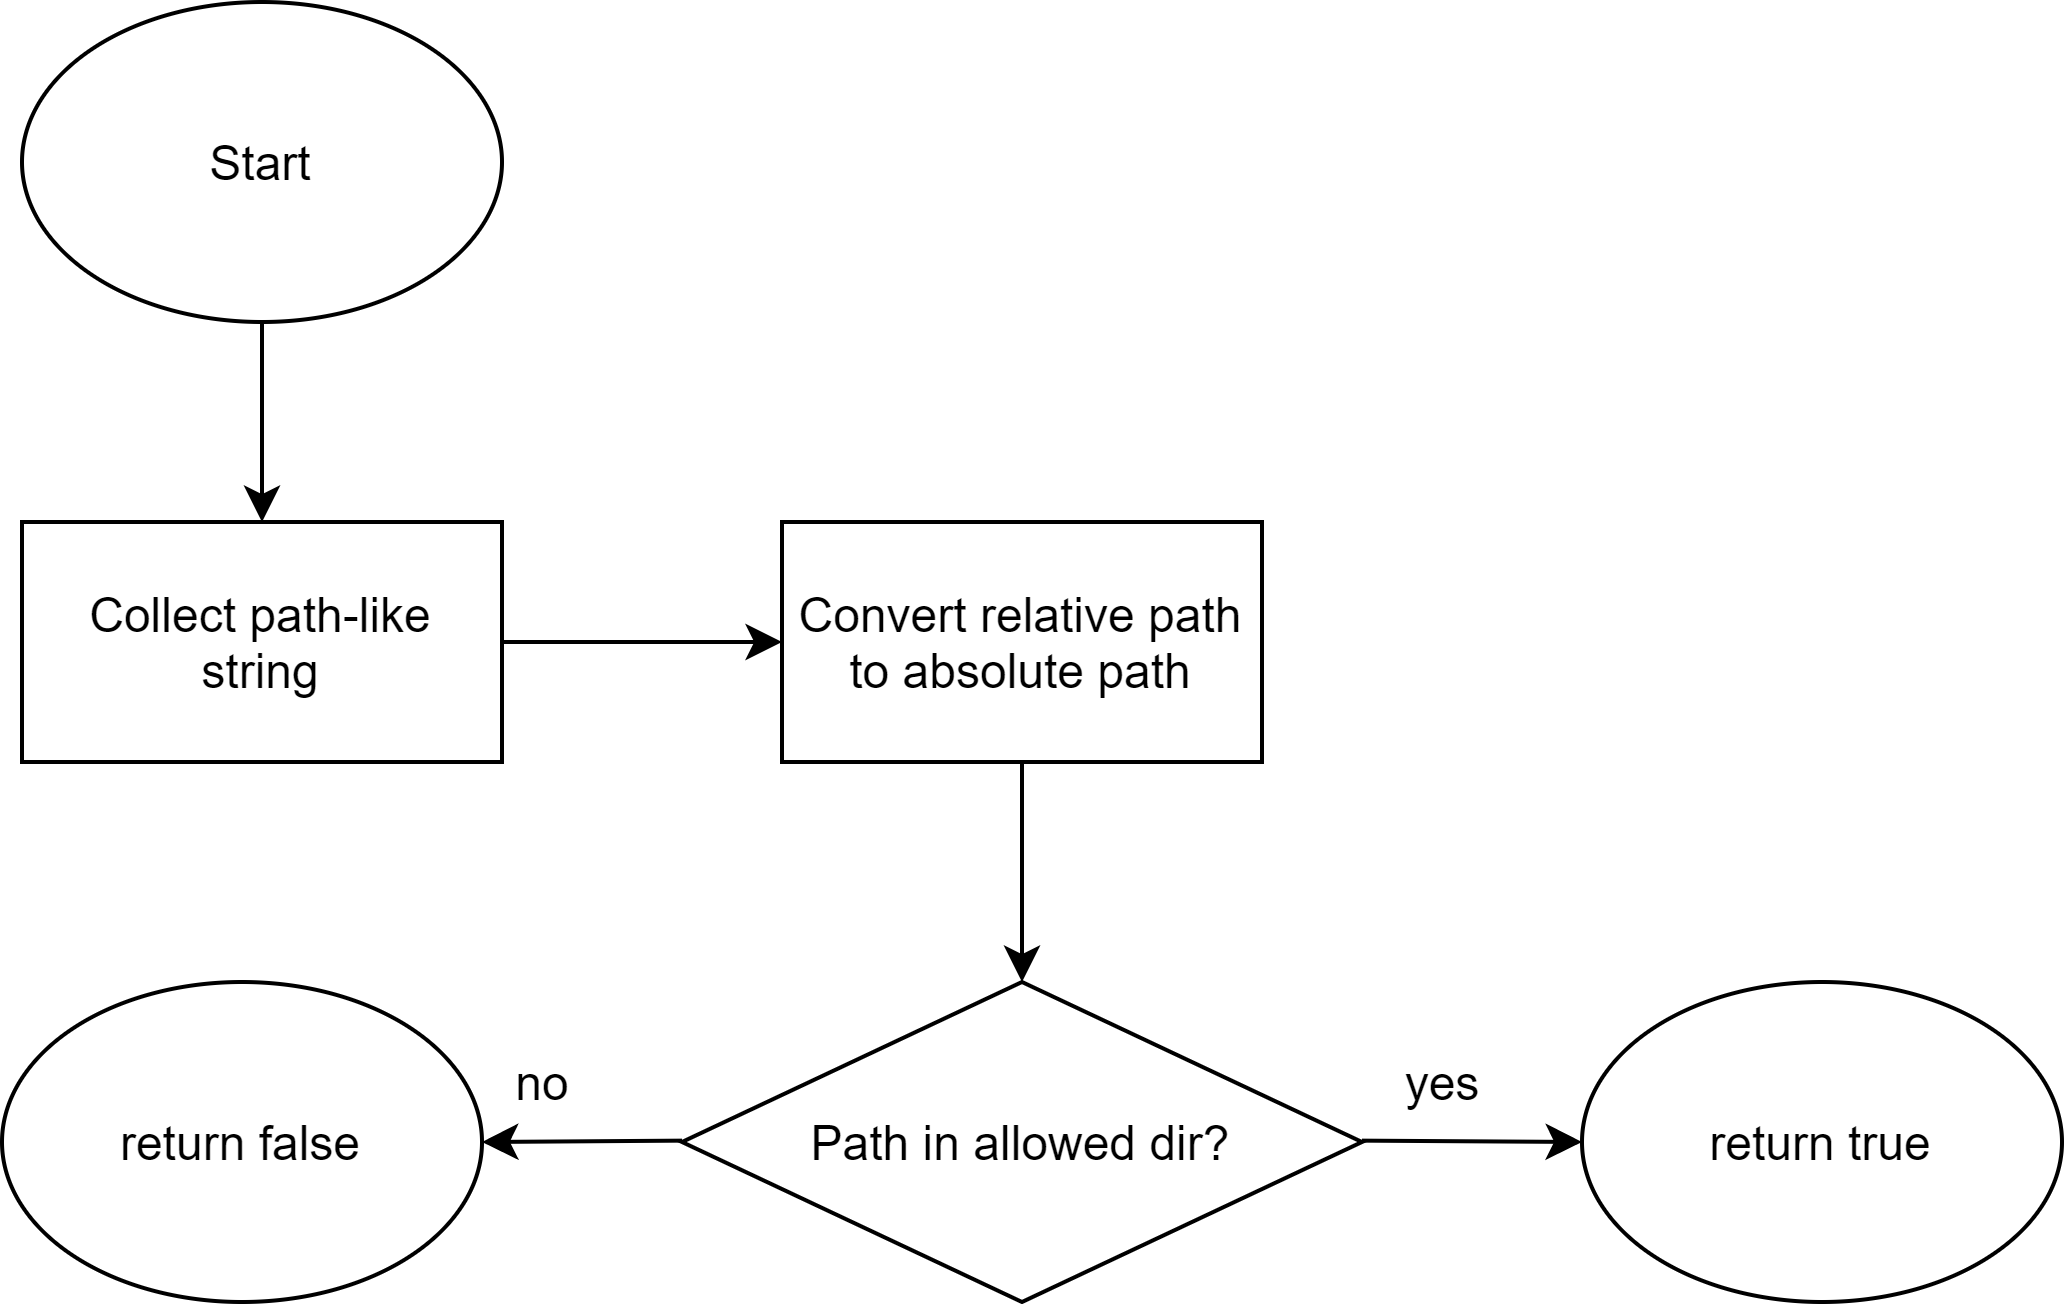
\includegraphics[width=0.9\linewidth]{images/algo_for_path_checking.png} 
      \caption{Algorithm for validating command parameters against directory whitelist} 
      \label{fig:algo_for_path_checking} 
      \vspace{4ex}
    \end{subfigure} 
    \caption{Policy for EXEC requests, and algorithm for validating command parameters}
    \label{fig3} 
\end{figure}


The policy used by the EXEC request checker is in Figure~\ref{fig:exec_policy}. Each privilege level possesses an allowlist of commands, "allowed\_cmd," and an allowlist of directories, "allowed\_dir." The command allowlist specifies what commands the user can issue, while the 
directory allowlist controls which directories a command can access. When an EXEC request is received, the EXEC checker examines all path-like strings in the command argument and verifies if they exist in the directory allowlist. If a command has no arguments, the EXEC checker checks whether the current working directory of 
the command is a subpath of a directory in the directory allowlist so that the command can only be executed in some specific directories. Notably, directory allowlist does not apply to terminal allocation commands like /bin/sh, /bin/bash, and sh. This permits users to allocate a terminal 
from any directory. For instance, the policy in Figure~\ref{fig:exec_policy} enables privileged users to issue cat, ls, and /bin/sh commands. The cat and ls commands are restricted to the /var directory and its subdirectories. Therefore, any attempt to execute commands in other directories (e.g., cat / and cat /bin) will be denied. 
On the other hand, since /bin/sh is included in the command allowlist, privileged users can allocate a terminal. Moreover, if a privilege level's command allowlist is empty, all commands issued by the user with this privilege level will be rejected.



The EXEC checker employs the algorithm presented in~\ref{fig:algo_for_path_checking} to validate the command parameters. It is important to note that the command and its arguments are conveyed as an array of strings from the user to the enclave. The first element of the array represents the command, and the subsequent elements 
correspond to the command's arguments. Consequently, the algorithm iterates through this array to inspect all the command's arguments, capturing absolute and relative paths. Absolute paths encompass strings beginning with '/,' whereas relative paths are the strings containing '.'' or '/'. Following 
this, the algorithm utilizes the command's current working directory to convert relative paths into absolute paths. Finally, it checks all paths against the directory allowlist. It returns false if a path is not a subpath defined in the policy.


\subsection{Protection for Privileged Exec Request}
\label{sec:design_prptect_privileged_request}
\begin{figure}[!htb]
    \centering
    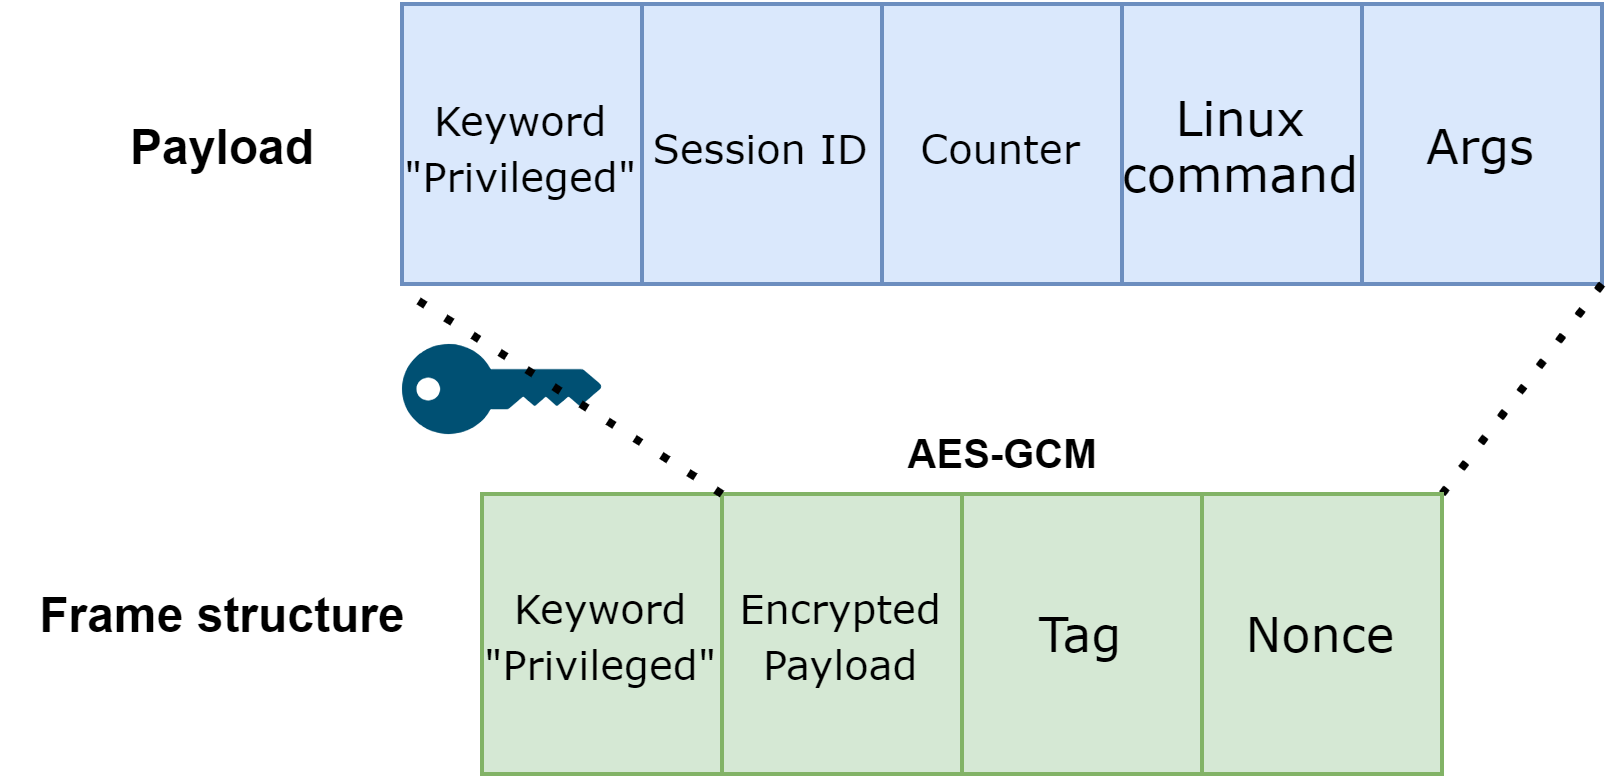
\includegraphics[width=0.4\textwidth]{images/exec_frame.png}
    \caption[Frame structure  for protecting privileged exec request]{Frame structure  for protecting privileged exec request}
    \label{fig:exec_frame}
\end{figure}
The frame structure shown in Figure~\ref{fig:new_pattern_of_exec} protects privileged commands and distinguishes them from non-privileged commands. The frame structure encapsulates the string "Privileged," the AES-GCM encrypted payload, the AES-GCM~\cite*{aes_gcm} random number (nonce) used for payload decryption, and the authentication tag. 
The plaintext payload contains the keyword "Privileged," the session ID, a counter,  a Linux command, and its parameters. Kubernetes and the OCI runtime specification require that commands and their parameters in EXEC requests be passed as a vector of strings. For example, ["cat", "/var/log"]~\cite*{k8s}. As such, 
the encrypted payload, nonce, and tag in the frame structure are encoded in base64, and the frame is passed as a string array to the enclave via the Kubernetes API. Note that the string array is part of the EXEC request process specification called args (See section\ref{subsec:oci_exec}). Upon receiving an EXEC request, 
the EXEC request checker can determine if the request is privileged by viewing the first element of the arg array. If the element is the keyword Privileged", the request will be classified as privileged.

AES-GCM~\cite*{aes_gcm} ensures the confidentiality, authenticity, and integrity of privileged commands and their arguments. Besides, it is easy to deploy, requiring only a shared key. After a successful remote attestation, a key is shared between the application owner and the enclave. The application owner can 
use this key to encrypt privileged commands and their parameters. When the enclave receives a privileged request, the EXEC request checker can use the key to confirm that the request was generated by a privileged user who knows the key (authentication), verify the request's integrity, and decrypt the 
request.


The monotonic counter and session are designed to prevent reply attacks. The counter is assigned by the enclave to a privileged user. When the value of the monotonic counter in an EXEC request is smaller than the reference value stored in the enclave, the request will be rejected. Since there may be 
more than one privileged user, it is hard to share the counter. Therefore, we introduce sessions. In this case, the enclave will assign each privileged user a random session id and a unique counter. This id and counter are stored in the enclave and will be sent to a privileged user via a secure channel. 
The privileged user can use the session id and counter to construct a privileged EXEC request. Note that the counter is added by one after each EXEC request. With the session and counter, we avoid the following two reply attacks. First, the attacker sends a request that belongs to an illegal session, 
i.e., the enclave does not store the session id. Second, the attacker has sent an outdated request to the enclave. This means that the counter value in a request is less than the current counter value recorded in the enclave for the requested session ID. In this case, the enclave will refuse to 
execute it.
\subsection{Session Assignment and Policy Updates}
\label{subsec:design_policy_session_update}
\begin{figure}[!htb]
    \centering
    
    \begin{minipage}{0.9\textwidth}
    \begin{subcolumns}[0.62\textwidth]
      \subfloat[Workflow of session assignment\label{fig:session_base_auth}]{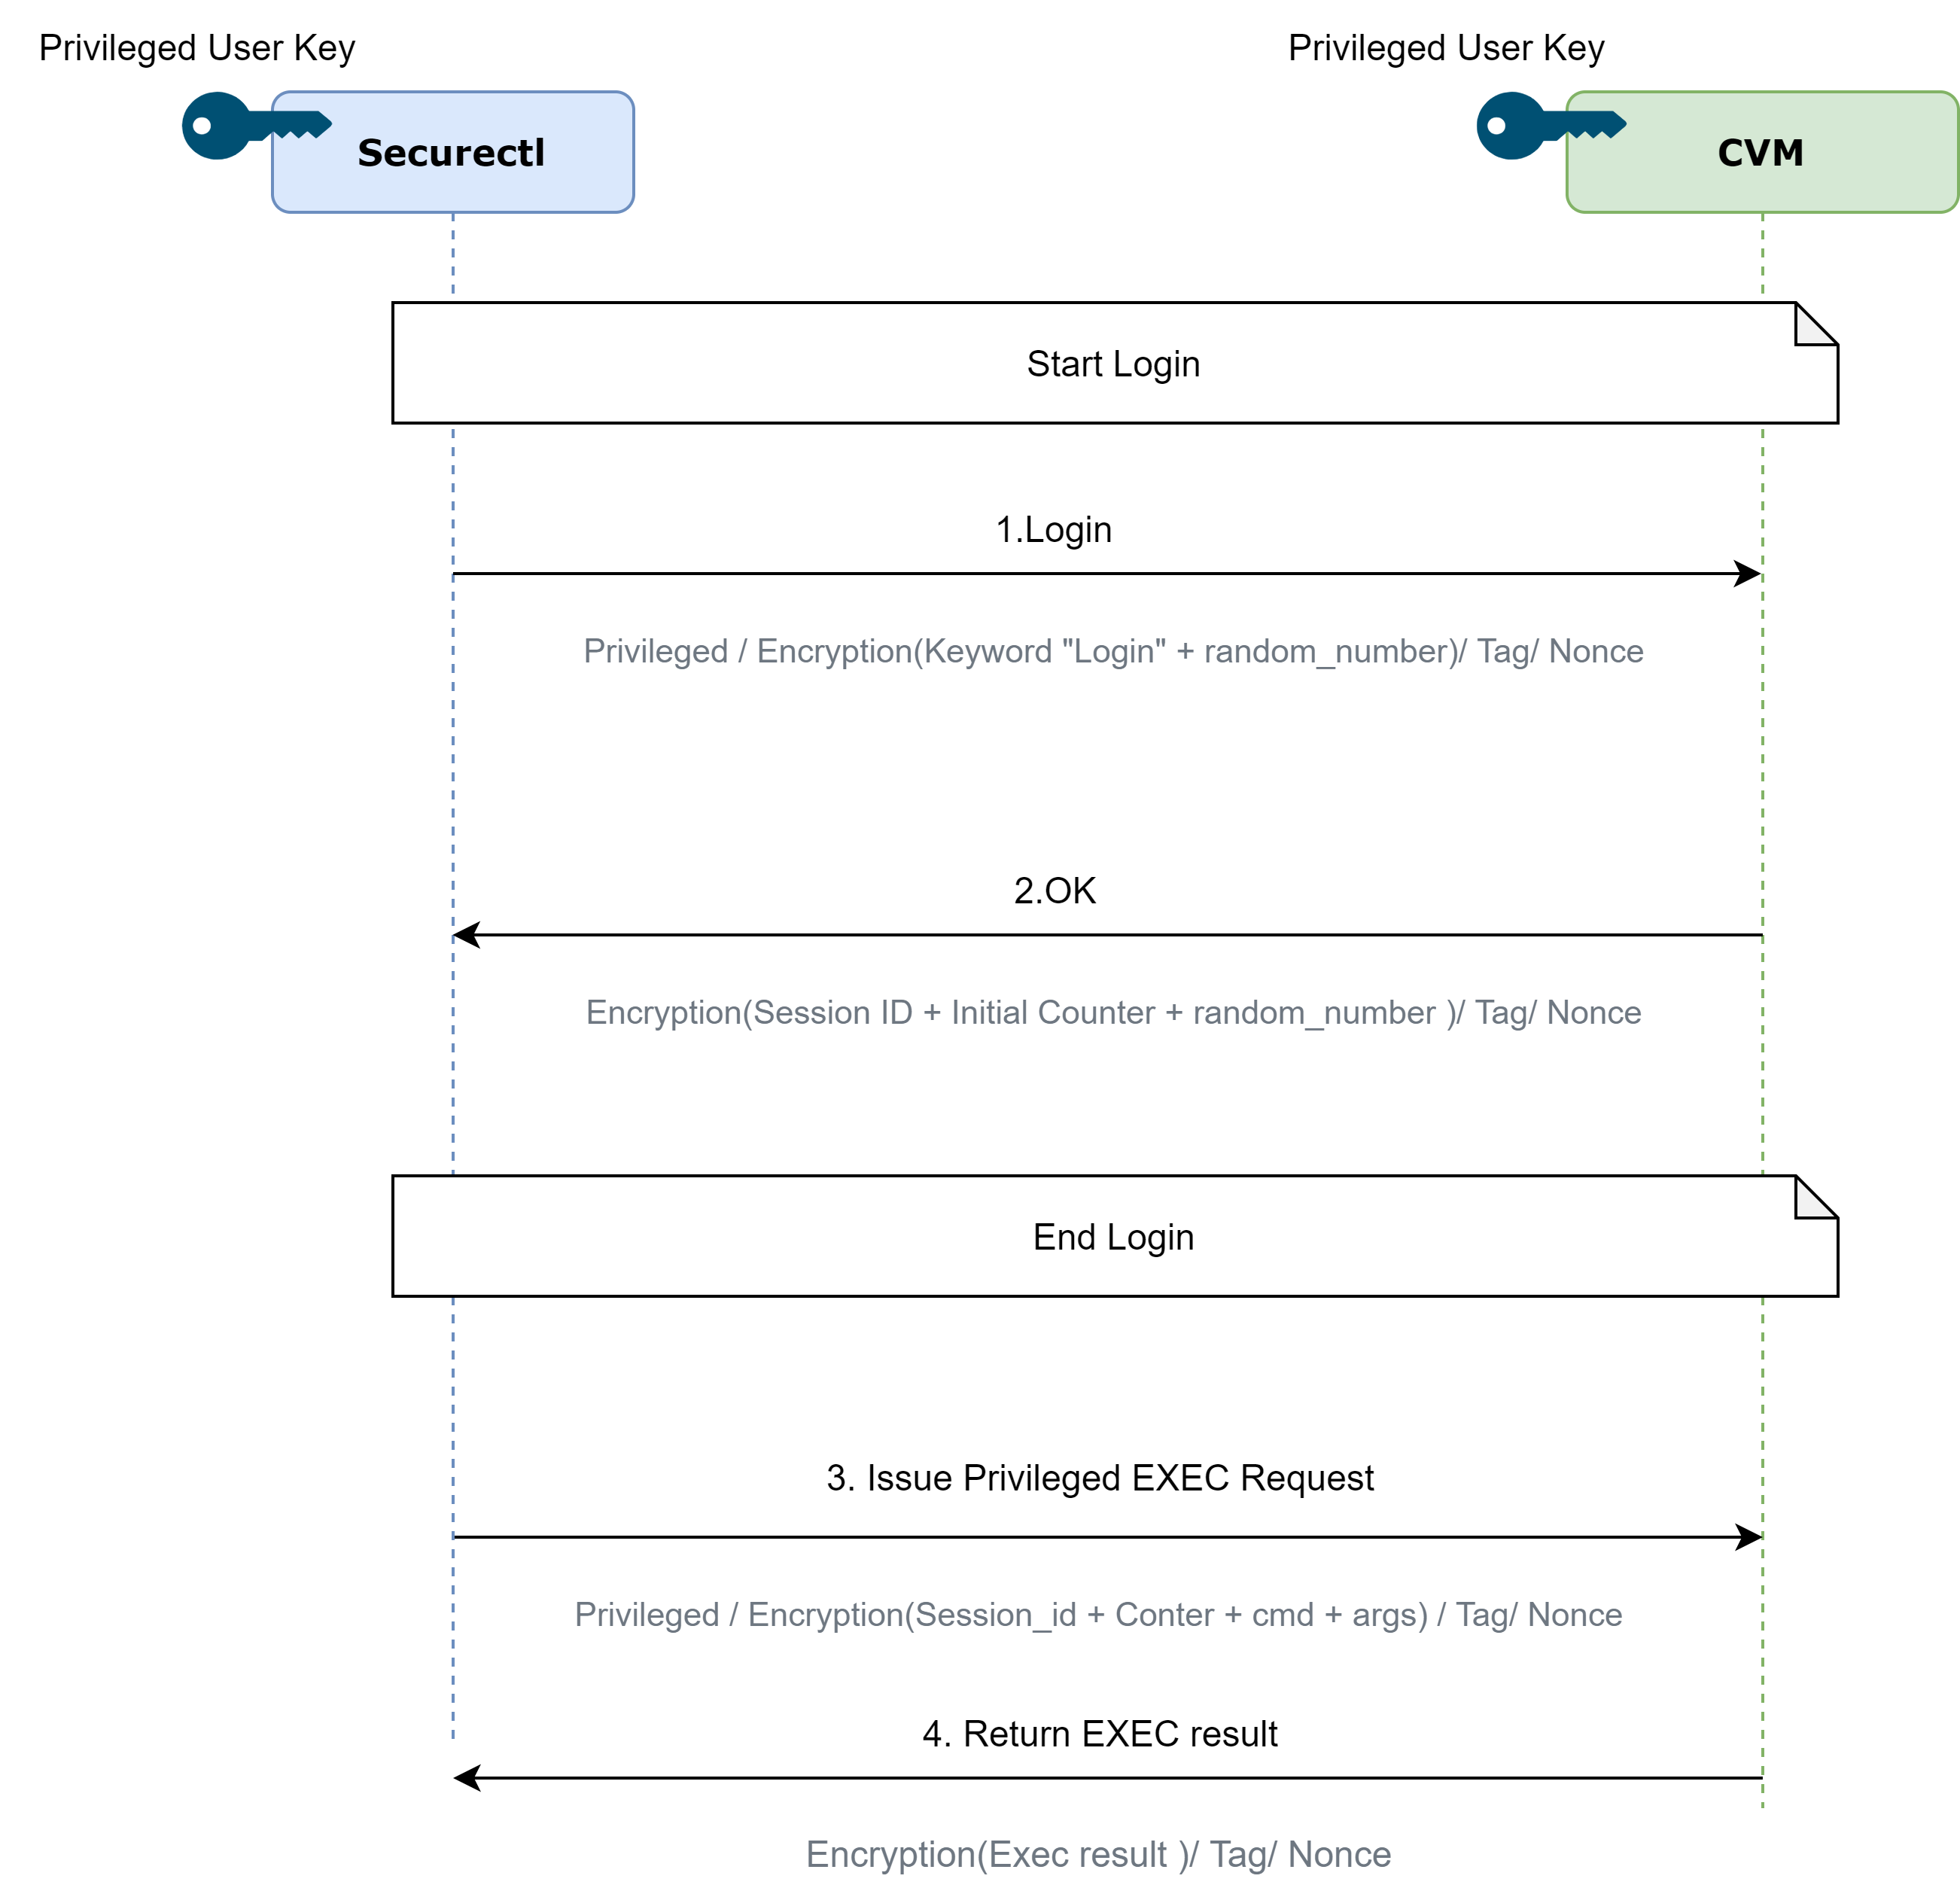
\includegraphics[width=\subcolumnwidth]{images/session_base_auth.PNG}}

    \nextsubcolumn[0.33\textwidth]
      \subfloat[Frame structure  for session allocation\label{fig:session_allocation}]{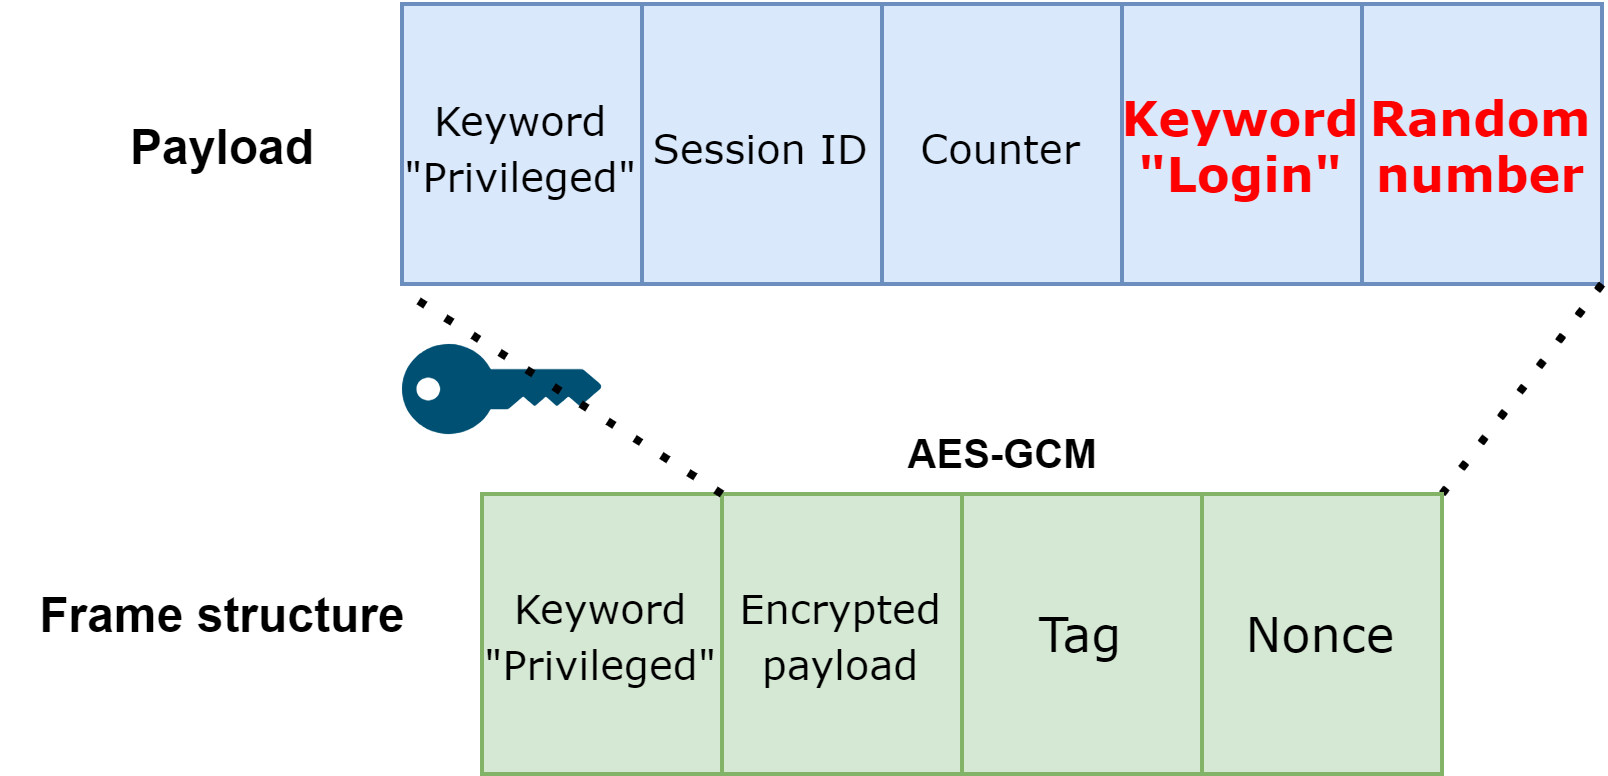
\includegraphics[width=\subcolumnwidth]{images/session_allocation.PNG}}

    \nextsubfigure
      \subfloat[Frame structure  for policy updates\label{fig:policy_frame}]{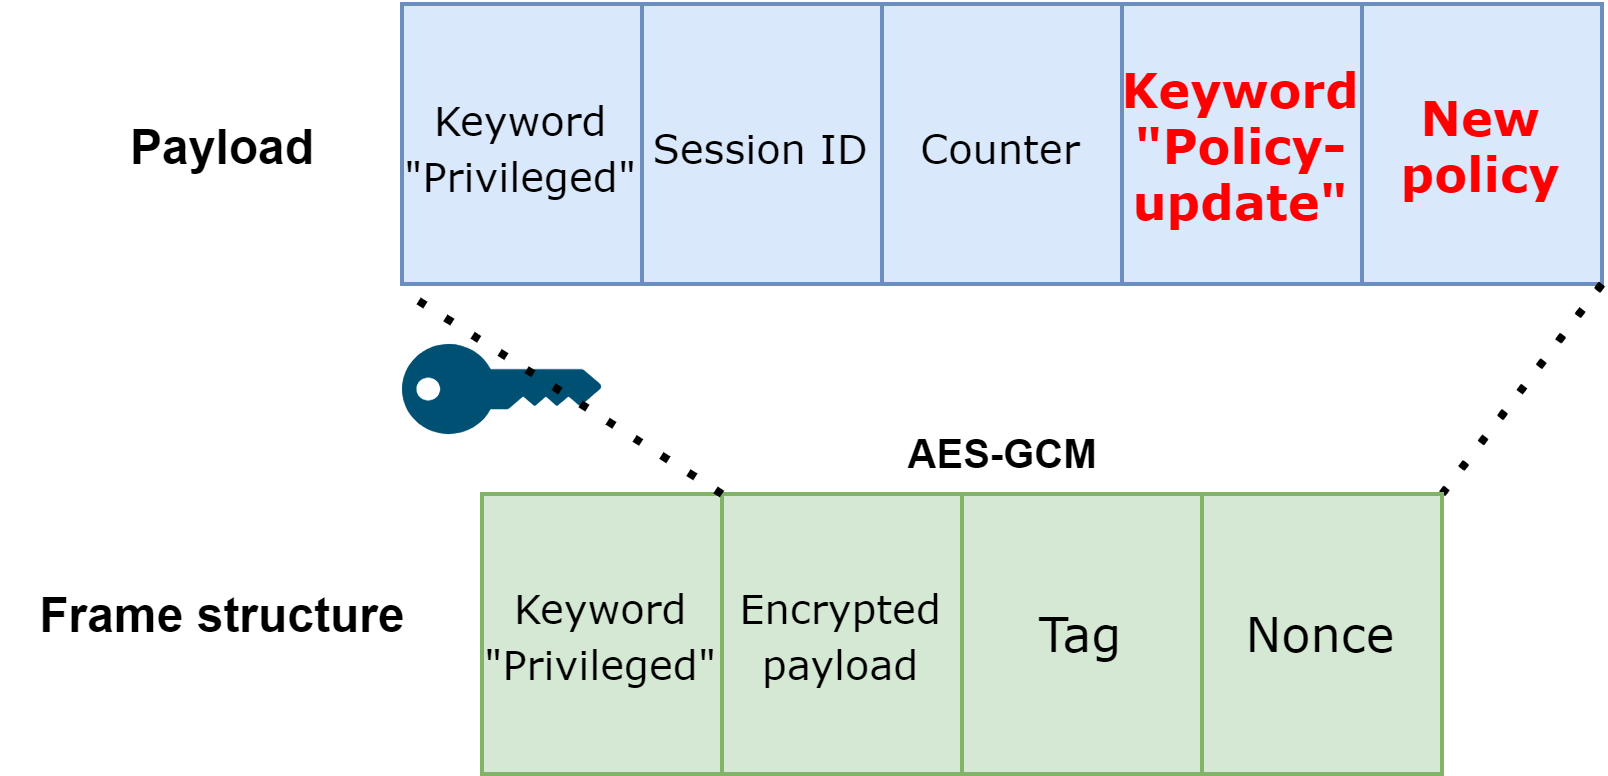
\includegraphics[width=\subcolumnwidth]{images/policy_frame.PNG}}
    \end{subcolumns}
    \end{minipage}
    
    \caption[Session Assignment and Policy Updates]{Session Assignment and Policy Updates}
    \label{fig:session_policy}
\end{figure}


Figure~\ref{fig:session_base_auth} demonstrates how a privileged user gets a session. The privileged user submits a login request using securectl in the login phase. The login request is a privileged EXEC request with the format visualized in Figure~\ref{fig:session_allocation}. Instead of an actual Linux command, the keyword Login and a random number 
are used as the command and parameter. The random number is used to prevent reply attacks. After the enclave verifies and decrypts the encrypted payload, it checks the command in the payload. If the command is the keyword Login, it assigns a session ID and a unique counter to the privileged user. 
These two values are stored in the enclave and returned to securectl securely. Specifically, it creates a process when that EXEC request is received. However, the keyword "Login" is not a Linux command. Thus, the enclave replaces the command executed by the EXEC process with" ls." Once the process 
completes running ls and writes the result to its STDOUT, the STDIO shield will intercept the data and replaces it with the session ID and counter. Since the login request is privileged, the STDIO shield will encrypt the data before sending it to the user. 

When the keyword "enabale\_policy" is true in the enclave policy, privileged users can use securectl to update the enclave policy. Similar to the session allocation request, the policy is updated by sending a privilege-level command to the enclave. The format of the command can be found in~\ref{fig:policy_frame}. Unlike 
the session request's payload, it uses the keyword policy-update as the command, with the new enclave policy as the command's argument

\section{Guest User Space Process STDIO Protection}
\label{sec:design_STDIO_PROTECTION}
We propose a guest user-space process STDIO shield to tackle the identified security issues (~\ref{vulnerabilities:2}, ~\ref{vulnerabilities:3}, ~\ref{vulnerabilities:6}). In the following, We explain how the STDIO shield protects both non-interactive and interactive processes. It is important to note that privileged processes refer to 
both the application process and processes executing privileged EXEC commands. The distinction between interactive and non-interactive processes lies in their STDIO, specifically whether it is of terminal type. 


\subsection{Distinguish the STDIO type of the Processes}
\label{sec:design_Distinguish_io}

The guest user space can accommodate various types of processes, including privileged-level non-interactive EXEC processes, privileged-level interactive EXEC processes, session or policy update processes, and various non-privileged-level EXEC processes. The STDIO shield handles the STDIO of these processes differently. For instance, 
to send the session id to a user, the shield intercepts the session process's STDOUT, replaces the content with the session ID assigned to the user, and encrypts it. Similarly, data written to the STDOUT and STDERR of privileged-level non-interactive processes is encrypted. Conversely, data belonging 
to non-privileged level process STDIO remains unaltered. Thus, the STDIO shield necessitates a mechanism for discerning between the various types of process STDIO.
 
The file descriptor representing the STDIO of a process cannot be used to distinguish between different processes' STDIO streams, as the file descriptors for STDIN, STDOUT, and STDERR are fixed as 0, 1, and 2, respectively. Qkernel, however, implements a virtual file system. Like the Linux kernel, each file descriptor in the Qkernel filesystem corresponds to 
a unique inode with a unique id. Therefore, the inode id can differentiate between the STDIO streams of different processes.
\begin{figure}[!htb]
    \centering
    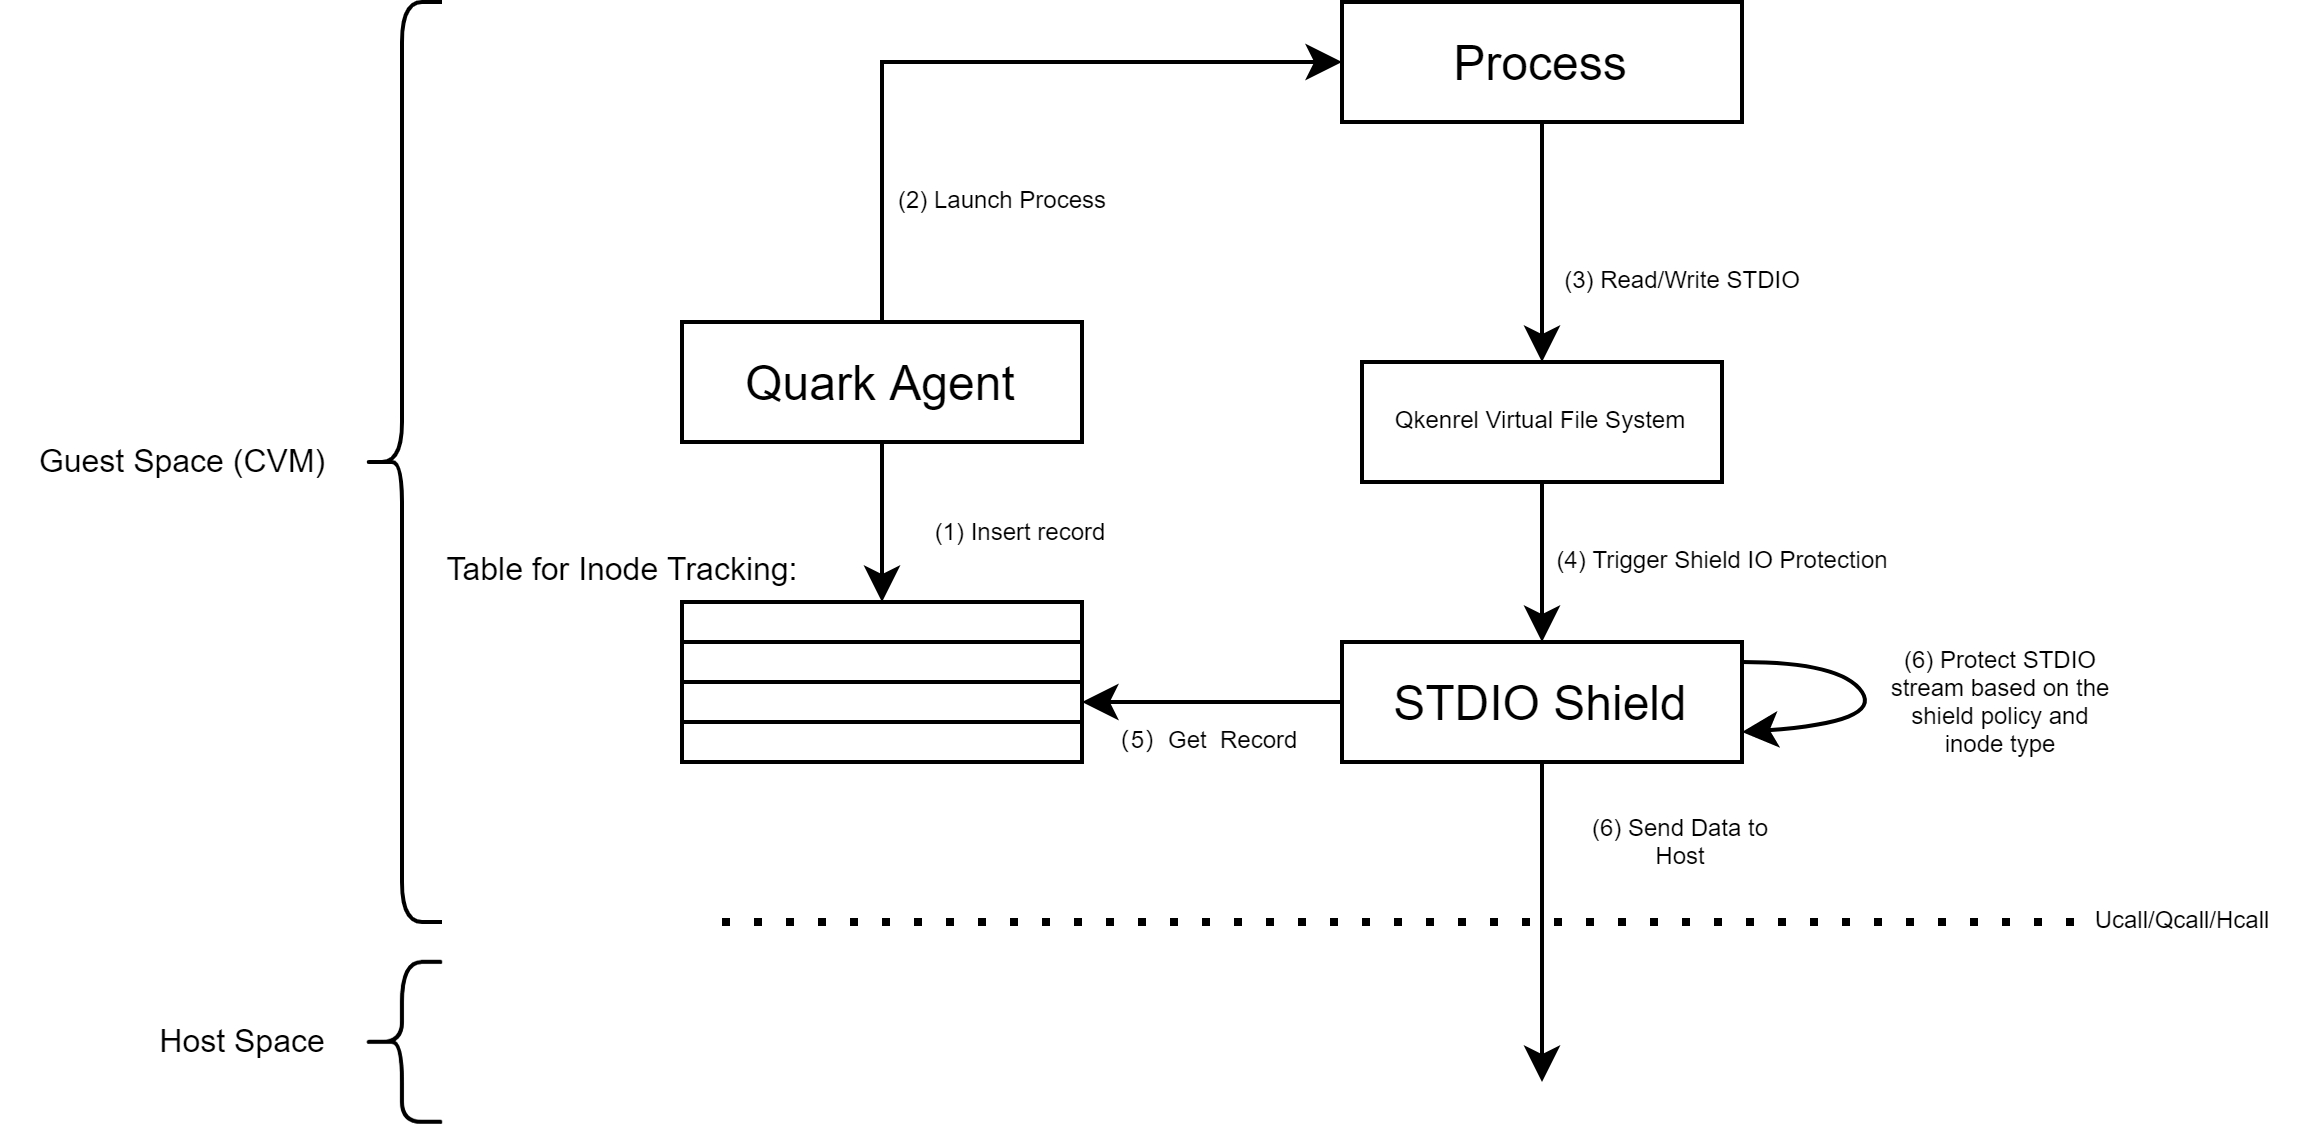
\includegraphics[width=0.8\textwidth]{images/differenciate_fds.png}
    \caption[Inode tracking table workflow]{Inode tracking table workflow}
    \label{fig:differenciate_fds}
\end{figure}
 
The STDIO shield maintains an inode table to track individual processes' STDIN, STDOUT, and STDERR. Each table entry records include the type of STDIO, the process's privilege level, the process type, and additional metadata. The available STDIO types consist of STDIN, STDOUT, and STDERR. Process privilege levels are classified as 
privileged or unprivileged. Process types encompass the application, interactive EXEC, non-interactive EXEC, policy update, and session assignment. An entry also includes a session ID and counter if the process type is the session assignment. Additionally, for policy update processes, the entry contains a boolean 
value indicating the success of the update. Like session assignment, the STDIO shield informs the user of the policy update result by substituting the data written to the STDOUT of the policy update process.

As shown in Figure~\ref{fig:differenciate_fds}, when the Quark agent creates a process and configures its STDIN, STDOUT, and STDERR file descriptors, corresponding records are created in the inode tracking table. When a process reads or writes its STDIO, the STDIO shield can locate the corresponding inode based on the file descriptor associated 
with the STDIO. By utilizing the inode id, the shield can retrieve the relevant record from the inode table and secure the data within the STDIO stream based on the shield policy.

\subsection{Non-interactive Process STDIO Protection}
\label{sec:design_non_interactive_stdio}
\begin{figure}[!htb]
    \centering
    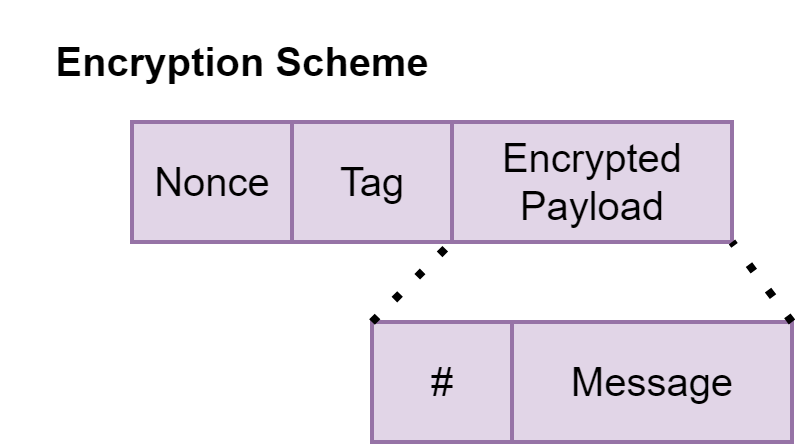
\includegraphics[width=0.3\textwidth]{images/normal_io_shiled_encryption_schema.png}
    \caption[Normal STDIO protection schema]{Normal STDIO protection schema}
    \label{fig:normal_io_shiled}
\end{figure}

Protecting the confidentiality and integrity of the data in the STDERR and STDOUT of privileged-level non-interactive processes is critical. To this end, the STDIO shield utilizes a frame structure in Figure~\ref{fig:normal_io_shiled} to cryptographically protect data written to the STDOUT and STDERR of these processes. The structure consists of an 
encrypted payload, a nonce, and an authentication tag. AES-GCM uses the nonce and the tag for decryption and authentication. The STDIO shield encrypts the payload using the key provided in the enclave policy. Since only the enclave and the enclave owner know the key, an attacker cannot decrypt the encrypted payload. Additionally, the use of AES-GCM ensures the 
confidentiality, integrity, and authenticity of the data. The plaintext payload comprises the data written into STDOUT or STDERR by these processes and a number used to prevent reorder or replay attacks. If a privileged user uses securectl to access an application’s logs, this number is utilized to verify whether the log has been reordered or lost. 
For privileged-level EXEC processes, this number is the counter’s value in the EXEC request. Upon receiving the EXEC result, securectl compares the reference value to the number in the payload to prevent replay attacks.


\subsection{Interactive Process STDIO Protection}
\label{subsec:design_terminal}


The goal is to ensure the confidentiality and integrity of the data within the STDIN, STDOUT, and STDERR streams of an interactive process. Achieving this requires end-to-end encryption and decryption of the process's STDIO. Specifically, the data written to STDIN is encrypted by the securectl on its side and decrypted within the enclave. Similarly, 
the STDOUT and STDERR data are encrypted within the enclave and decrypted by the securectl. As discussed in Section~\ref{sec:security_analyse_STDIO}, Quark uses the terminal I/O redirection thread in Quark Shim, and the host TTY drive to facilitate the terminal STDIO handling. Since the data written by securectl to STDIN is encrypted, the terminal 
I/O redirection thread cannot filter signals.

For this reason, the terminal I/O redirection thread is merged into the STDIO shield in the enclave. Upon receiving the encrypted data, the STDIO shield reads it from the named pipe representing the process's STDIN, decrypts it, and filters out possible signals. The remaining data is then forwarded to the TTY master for further processing. It is important 
to note that the data written to the host TTY driver must be encrypted since the enclave does not trust the host. However, this encryption significantly impacts performance and causes data written to the host TTY driver not to be processed correctly, leading to a malfunctioning terminal.

\begin{figure}[!htb]
    \centering
    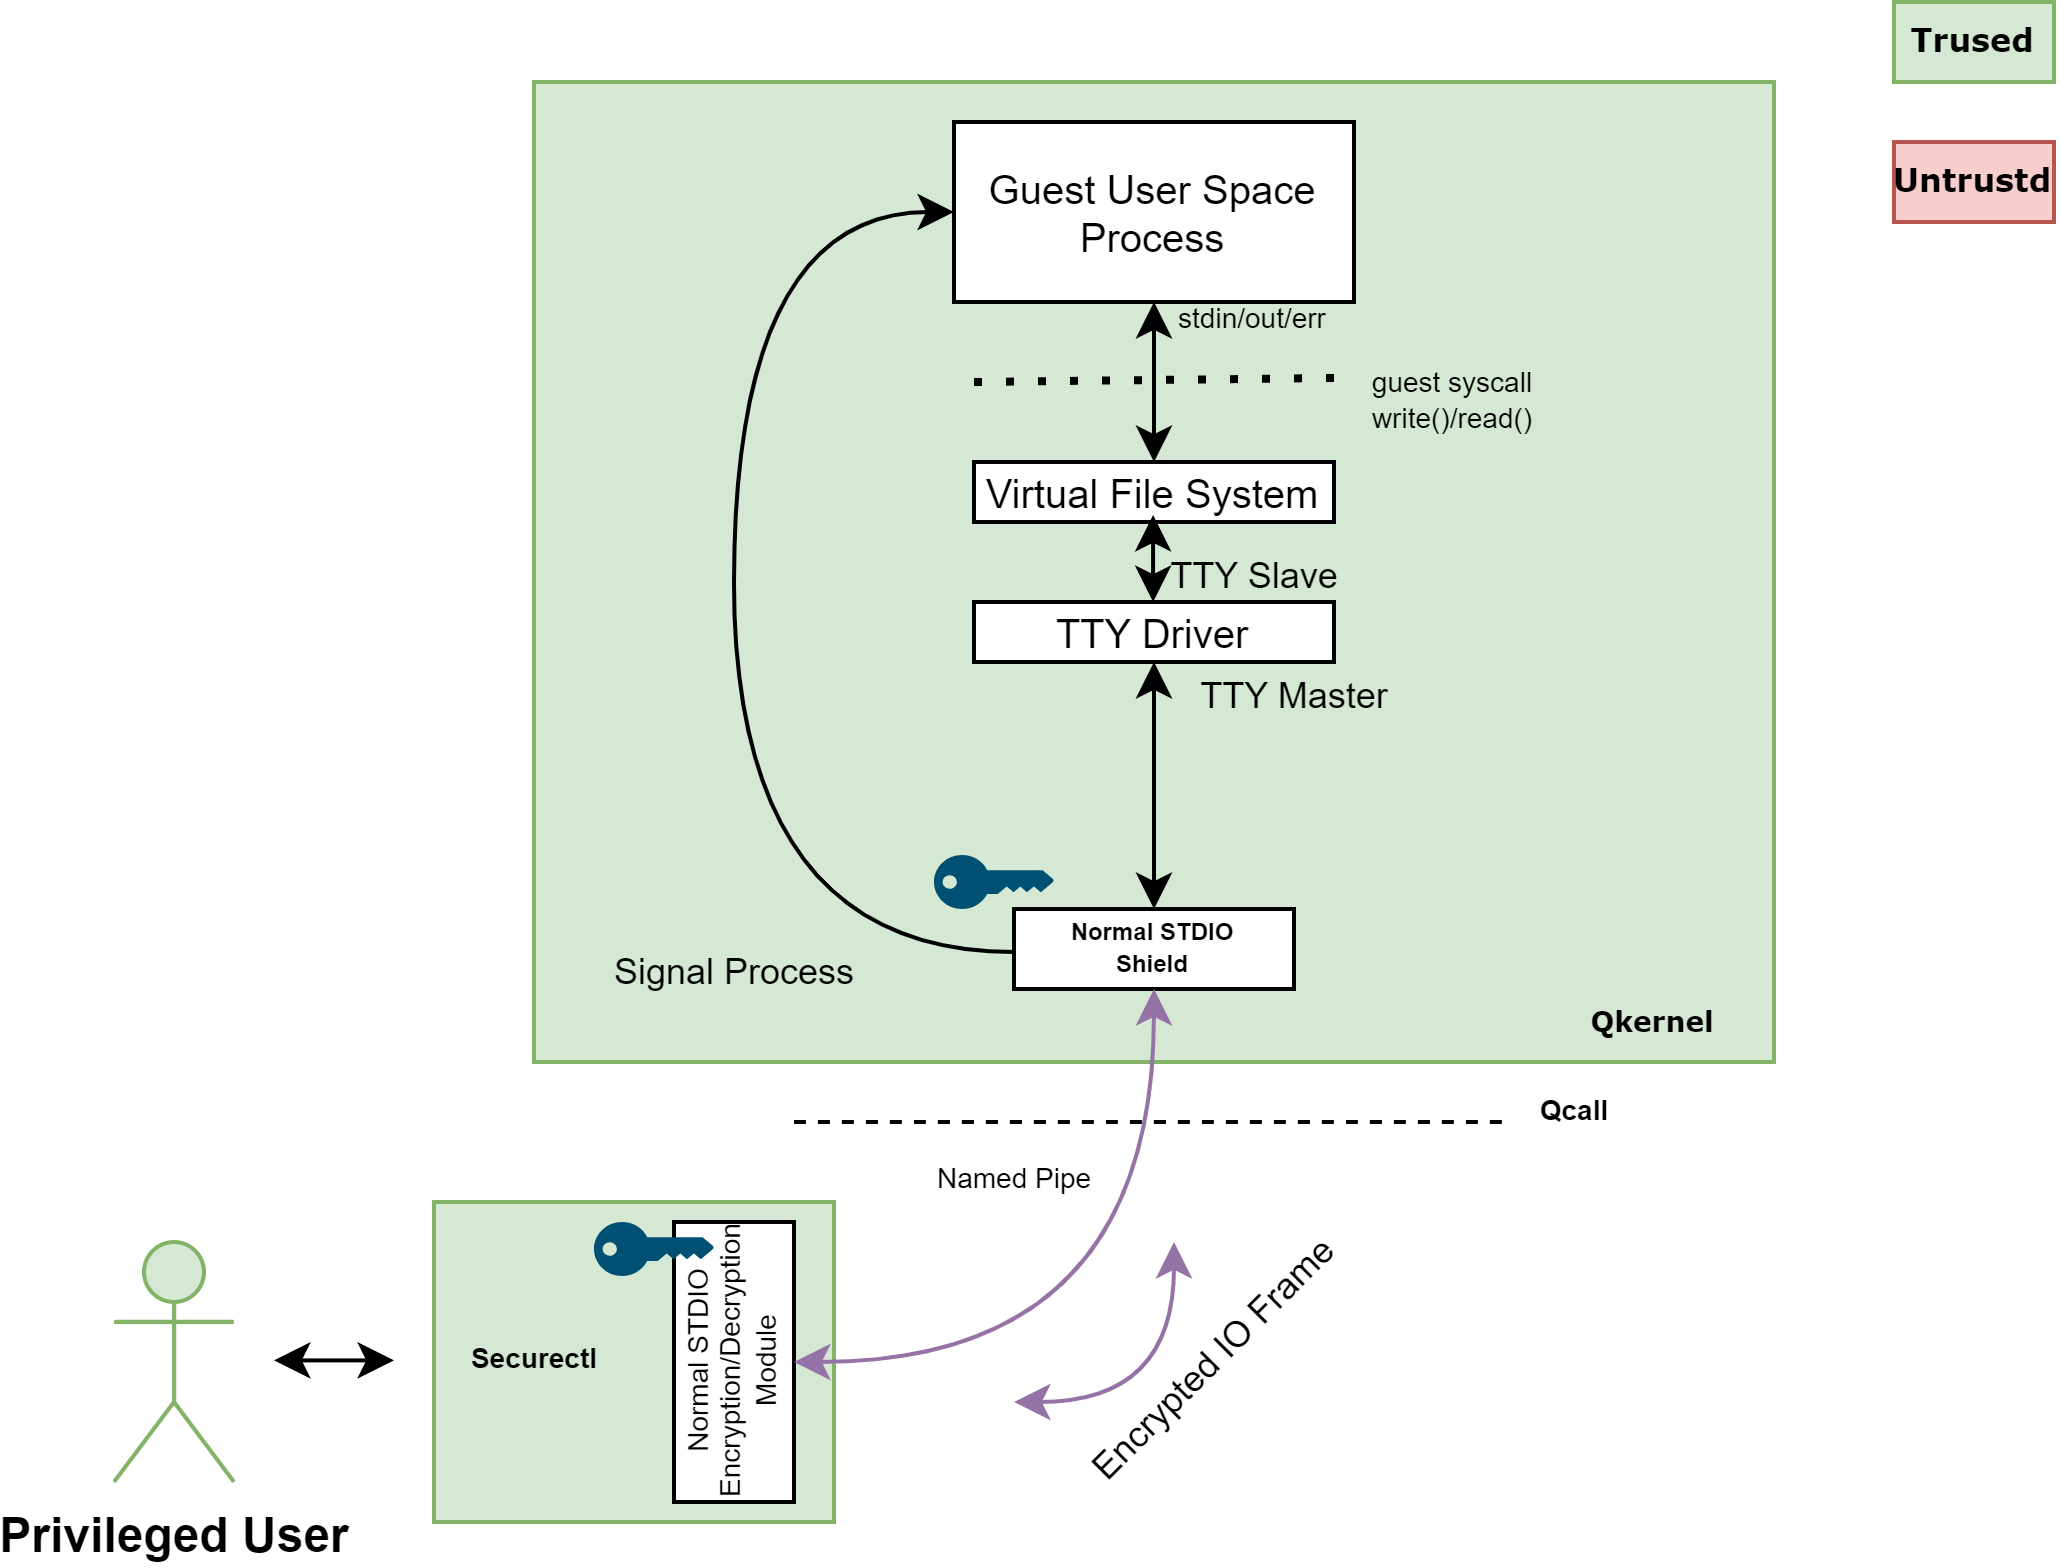
\includegraphics[width=0.6\textwidth]{images/terminal_shiled3.png}
    \caption[Terminal STDIO Protection in case of using Qkernel TTY driver]{Terminal STDIO Protection in case of Qkernel TTY driver}
    \label{fig:terminal_shiled3}
\end{figure}

To address this problem, as depicted in Figure~\ref{fig:terminal_shiled3}, a TTY driver must be implemented in the enclave that functions similarly to the host kernel TTY driver. This TTY driver will handle character echoes, conversion between line feeds and carriage returns, and buffering data written to the TTY master. For instance, when a guest userspace 
process writes data to its STDOUT, the write system call handler will redirect the data to the Qkernel TTY driver. The TTY driver processes the data, transmits it to the TTY master, and then alerts the shield to initiate further processing. Following that, the shield encrypts the data extracted from the TTY master and transfers it through the Qcall interface to 
securectl.  Securectl then decrypts the data before transmitting it to the user terminal. On the other hand, upon receiving data from the STDIN-named pipe, the STDIO shield decrypts it and forwards the decrypted data to the TTY driver for further processing. When the user presses '\textbackslash r,' the TTY driver transfers its buffered data to the interactive process. It is important to note 
that the STDIO shield applies the same data encryption scheme to both the interactive and non-interactive processes' STDIO.

\subsection{Limitations and Policy for STDIO Shield}
The design of Section~\ref{subsec:design_terminal} has yet to be implemented due to the complexity of the interactive process shield. Consequently, this poses two issues. Firstly, the logs of the interactive application are in plaintext. Secondly, anyone can attach to the interactive application and execute commands. Therefore, as a temporary mitigation, the data written to the STDOUT 
and STDERR of the interactive application process is encrypted using the schema outlined in Section~\ref{sec:design_non_interactive_stdio}. This ensures that the interactive application's logs are encrypted. Although an attacker could attach to an interactive application and issue commands, they would not gain any valuable information because the results returned by the application are encrypted.
 
Currently, the STDIO shield will encrypt the STDIO of userspace processes based on the enclave policy depicted in Figure~\ref{fig:stdio_policy}. If no\_interactive\_process\_stdout\_err\_encryption is true, the STDIO shield will encrypt the STDOUT and STDERR of all 
non-interactive privilege processes. When interactive\_porcess\_stdout\_err\_encryption is true, the STDIO Shield encrypts STDOUT and STDERR for interactive privilege processes.

\begin{figure}[!htb]
    \centering
    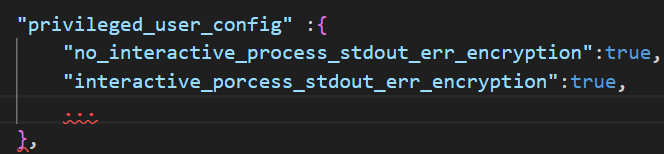
\includegraphics[width=0.6\textwidth]{images/stdio_policy.png}
    \caption[Policy for STDIO shield]{Policy for STDIO shield}
    \label{fig:stdio_policy}
\end{figure}


\section{System Call Interceptor}
\label{sec:design_Interceptor}
\begin{figure}[!htb]
    \centering
    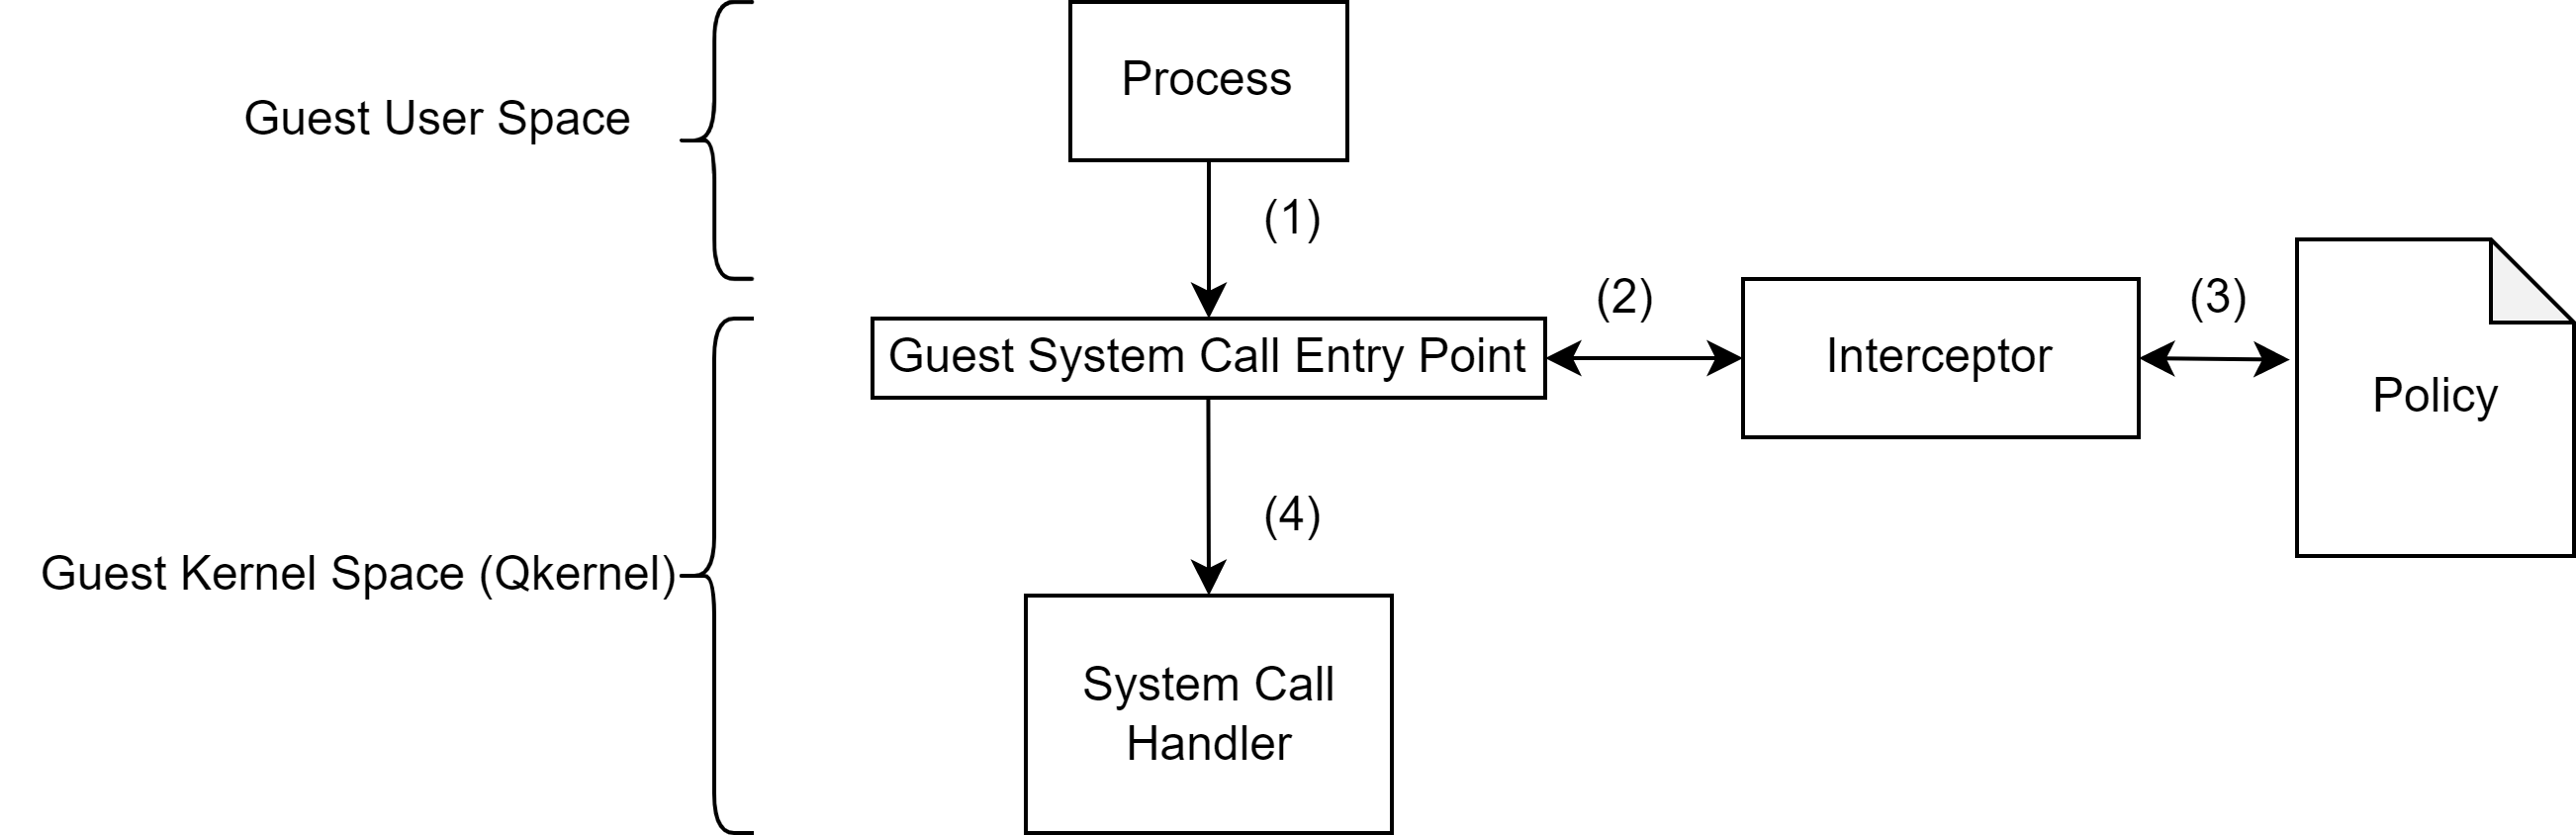
\includegraphics[width=0.8\textwidth]{images/syscall_interceptor.png}
    \caption[System call interceptor workflow]{System call interceptor workflow}
    \label{fig:syscall_interceptor}
\end{figure}
A system call interceptor is implemented in Qkernel, as illustrated in Figure~\ref{fig:syscall_interceptor}. When a guest system call is invoked, the CPU jumps to the guest system call entry point. This entry point is responsible for finding the system call handler in the Qkernel based on the system 
call ID. However, before it does so, it must call the interceptor. The interceptor decides whether the system call is allowed based on the shielding layer's policy. If the system call is not permitted, the guest system call entry point returns EPERM instead of calling the 
system call handler.

\begin{figure}[!htb]
    \centering
    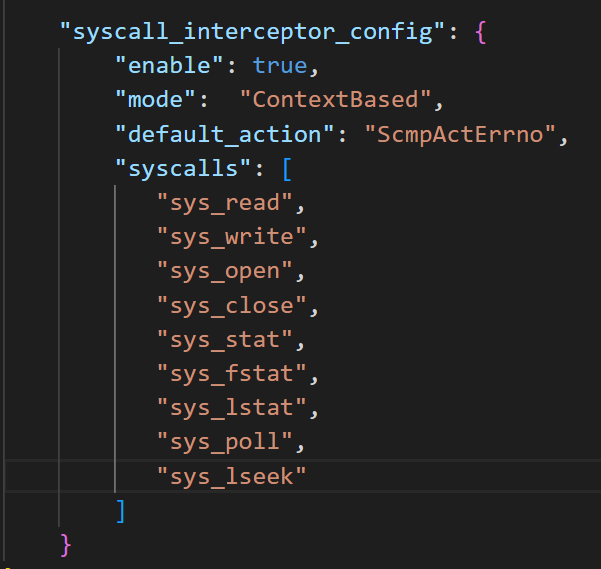
\includegraphics[scale=0.4]{images/policy_system_call.png}
    \caption[System call interceptor's policy]{System call interceptor's policy}
    \label{fig:policy_system_call}
\end{figure}

The interceptor policy is part of the enclave policy and is displayed in Figure~\ref{fig:policy_system_call}. The keyword "enable" determines whether the interceptor is enabled. The keyword mode specifies the system interceptor's mode: ContextBased or GlobalBased. In GlobalBased mode, the interceptor 
functions across all guest processes, while in ContextBased mode, it operates exclusively for the application process. Considering the potential presence of multiple processes in the guest user space, it is strongly recommended to employ GlobalBased mode. Currently, the system 
interceptor supports only the action, ScmpActErrno, which entails rejecting system calls when their IDs are absent from the allowlist termed "syscalls."





\section{Qkernel Log Manager}
\label{sec:Qkernel_logger}
A Qkernel log manager is implemented to address issue \ref{vulnerabilities:12}. It can be configured utilizing the enclave policy, exemplified in Figure~\ref{fig:qkernel_Log_config}. The keyword enabled determines whether the manager is enabled. When set to false, the Qkernel log system employs the logging level specified in 
the Qkernel configuration file. Furthermore, the keyword "allowed\_max\_log\_level" designates the maximum log level Qkernel can print. As discussed in Section~\ref{sec:Qkernel_Log_Misconfiguration}, Qkernel supports five log levels. For instance, when "allowed\_max\_log\_level" is set to INFO, Qkernel is exclusively restricted to printing 
logs at the INFO and ERROR levels. Additionally, the enclave policy is passed to the enclave during application deployment. Notably, the Qkernel log manager is enabled and employs the log level OFF before the enclave obtains the policy from the secret manager.
\begin{figure}[!htb]
    \centering
    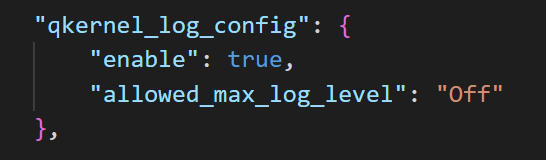
\includegraphics[width=0.4\textwidth]{images/qkernel_Log_config.png}
    \caption[Qkernel log manager's policy]{Qkernel log manager's policy}
    \label{fig:qkernel_Log_config}
\end{figure}

\section{Modification to OCI}
\label{sec:Modification_OCI}

\subsection{Extending the container lifecycle to support confidential computing}
The container lifecycle definition in the OCI RUNTIME specification~\cite*{oci-runtime-spec} lacks support for confidential computing. In this section, we first define container runtime and enclave in the context of confidential computing. Then we will propose modifications to the container 
lifecycle.


\subsubsection{Definition of Runtime and Enclave in Confidential Computing}

Currently, the container runtime in the OCI runtime specification~\cite*{oci-runtime-spec} refers to the runtime environment used to create containers. A VM-based container runtime includes the shim process, the hypervisor, and the agent inside the guest used to create and manage containers. 
For example, in the Kata containers~\cite*{Kata-Containers}, these three components correspond to kata-shim, qemu, and kata-agent, respectively. However, in confidential computing, the runtime is divided into two parts: the trusted agent, the untrusted shim process, and the hypervisor. Therefore, we redefine 
the runtime as untrusted runtime components, including the shim and hypervisor. In addition, we refer to the guest as an enclave containing the agent, guest kernel, etc.

\subsubsection{Modification to Container Lifecycle}
We make the following changes to the container lifecycle. Note that the bold text in the list is the part we modified; the rest is copied from OCI runtime specification~\cite*{oci-runtime-spec}.

\begin{enumerate}
    \item OCI compliant runtime's create command is invoked with a reference to the location of the bundle and a unique identifier.
    \item The container's runtime environment and enclave MUST be created according to the configuration in config.json. If the runtime is unable to create the environment specified in the config.json, it MUST generate an error. While the resources requested in the config.json MUST be created, the user-specified program (from process) MUST NOT be run at this time. Any updates to config.json after this step MUST NOT affect the container
    \item The prestart hooks MUST be invoked by the runtime. If any prestart hook fails, the runtime MUST generate an error, stop the container, and continue the lifecycle at step 16
    \item The createRuntime hooks MUST be invoked by the runtime. If any createRuntime hook fails, the runtime MUST generate an error, stop the container, and continue the lifecycle at step 16.
    \item The createContainer hooks MUST be invoked by the runtime. If any createContainer hook fails, the runtime MUST generate an error, stop the container, and continue the lifecycle at step 14.
    \item Runtime's start command is invoked with the unique identifier of the container.
    \item The startContainer hooks MUST be invoked by the runtime. If any startContainer hook fails, the runtime MUST generate an error, stop the container, and continue the lifecycle at step 14.
    \item \textbf{The Enclave receives the runtime’s start request and constructs a process for the user-specified program. If this hook fails, the enclave MUST generate an error, stop the container, and continue the lifecycle at step 16}
    \item \textbf{The enclave MUST invoke the application launch measurement hook if the user-specified program’s binary is loaded from the host. If this hook fails, the enclave MUST generate an error, stop the container, and continue the lifecycle at step 16.}
    \item \textbf{The attestation and provisioning hook MUST be invoked within the enclave when the enclave finish loading the program’s binary. If this hook fails, the enclave MUST generate an error, stop the container, and continue the lifecycle at step 16.}
    \item \textbf{The application process enters user space and starts to run.}
    \item \textbf{The enclave MUST invoke the runtime measurement hook when the program process loads binary or shared library from the host. If this hook fails, the enclave MUST generate an error, stop the container, and continue the lifecycle at step 16}
    \item \textbf{The enclave MUST invoke the STDIO protection hook when the program/exec process reads or writes data from its standard IO. If this hook fails, the enclave MUST generate an error, stop the container, and continue the lifecycle at step 16}
    \item The poststart hooks MUST be invoked by the runtime. If any poststart hook fails, the runtime MUST log a warning, but the remaining hooks and lifecycle continue as if the hook had succeeded.
    \item The container process exits. This MAY happen due to erroring out, exiting, crashing, or the runtime's kill operation being invoked.
    \item Runtime's delete command is invoked with the unique identifier of the container.
    \item The container MUST be destroyed by undoing the steps performed during create phase (step 2).
    \item The poststop hooks MUST be invoked by the runtime. If any poststop hook fails, the runtime MUST log a warning, but the remaining hooks and lifecycle continue as if the hook had succeeded.    
  \end{enumerate}

  

  The application launch measurement hook should be called when the enclave loads the application binary from the host. This hook must be executed in the enclave namespace. It measures the binaries loaded from the host before the application process starts. The attestation and provisioning hook will add the measurement result to attestation evidence and then 
  forward it to the relying party for integrity check. Note that the \acrshort{TEE} hardware must measure this hook as part of the enclave container runtime component.
 
  The attestation and provisioning hook must be invoked after the enclave loads the application binary but before the application process stack is set. The enclave uses this hook to authenticate itself to the relying party and retrieve the secrets. A reference design can be found in Section~\ref{sec:secure_application_deployment}. Note that this hook must be 
  executed in the enclave namespace. After the attestation and provisioning hook retrieves the secrets, the environment variable and application parameter type secrets should be pushed into the application process's stack. The enclave should store the file type secret in a trusted environment, such as enclave memory. 
   
   
  The enclave should call the runtime measurement hook when the application loads a shared library or binary file from the host at runtime. This hook must be executed in the enclave namespace. It forces the integrity check on the loaded shared library or binary against a reference value obtained from relying party.    
   
   
  The STDIO protection hook should be invoked when an application or a privileged exec process reads or writes its STDIO. It encrypts the privileged process's STDIN, STDOUT, and STDERR based on policy obtained from relying party. A reference design can be found in Section~\ref{sec:design_STDIO_PROTECTION}.
   
  The attestation and provisioning hook, runtime measurement hook, and STDIO protection hook may be included as part of the enclave's operating system or loaded from the host after the enclave starts. In the former case, these hooks will be measured by the \acrshort{TEE} hardware or bootloader. In the latter case, The application launch measurement hook should measure 
  these hooks. 
\subsection{EXEC Operating Guidelines}
\label{subsec:oci_exec}
The OCI runtime specification intentionally refrains from standardizing the EXEC operation to provide developers with flexibility~\cite*{exec_semantics}. However, in confidential computing scenarios, the EXEC operation allows attackers to acquire application secrets, thereby compromising confidentiality. As a result, we advocate for the 
standardization of the EXEC operation.
 
We utilize the proposal depicted in Figure~\ref{fig:exec_propose} as a foundation for standardization. This proposal was initially submitted to the OCI runtime spec forum, although it was ultimately not accepted due to the previously outlined reason.
 
\begin{figure}[!htb]
    \centering
    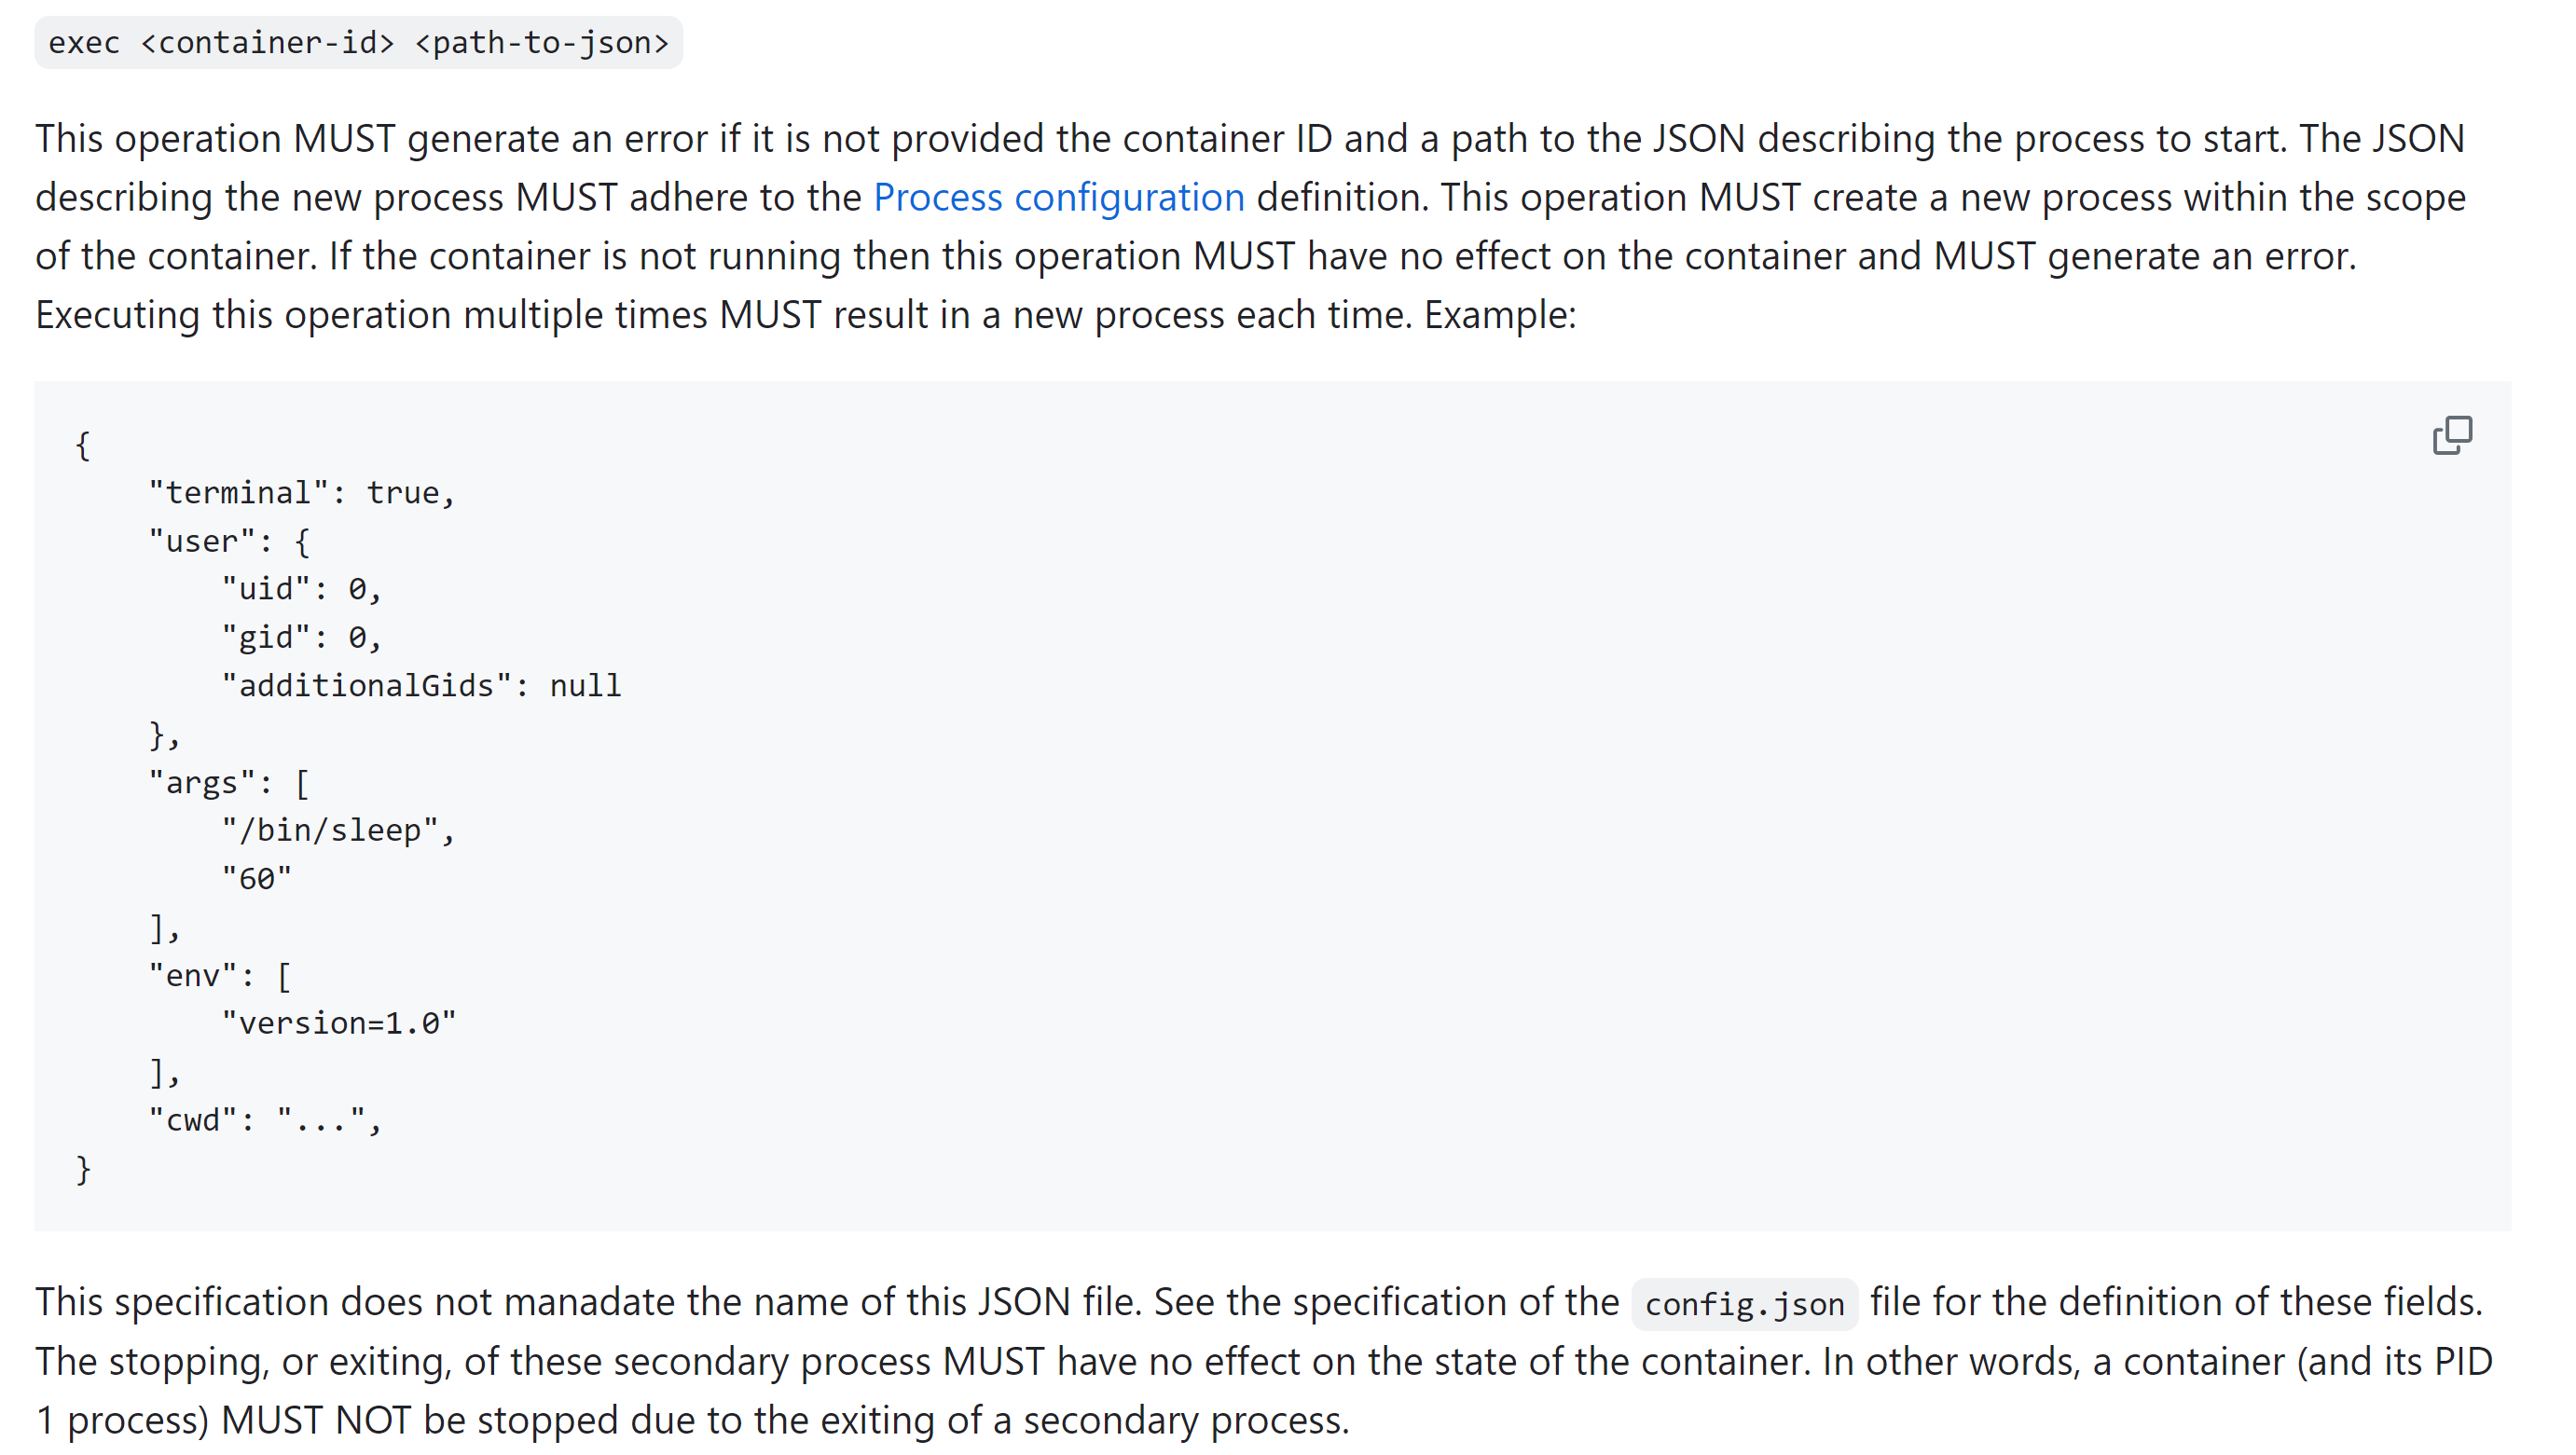
\includegraphics[width=0.8\textwidth]{images/exec_propose.png}
    \caption[Proposal for standardizing EXEC operation]{Proposal for standardizing EXEC Operation from~\cite*{exec_proposal} }
    \label{fig:exec_propose}
\end{figure}
 
In the confidential computing scenario, EXEC requests should be categorized into privileged requests issued by the application owner and unprivileged requests issued by others. The method discussed in Section~\ref{sec:design_prptect_privileged_request} is employed to protect the args array in the EXEC specification (Figure~\ref{fig:exec_propose}). This way, 
we can differentiate between privileged and non-privileged requests and ensure the confidentiality and integrity of privileged commands. This method necessitates sharing a symmetric key between the privileged user and the enclave. The enclave can obtain this key through the remote attestation and provisioning hook. Prior to creating an EXEC process,
the enclave must authenticate and control access to the request based on the policy shown in Figure~\ref{fig:exec_policy}. The authentication and access control workflow can be found in section~\ref{sec:impl_exec}. Additionally, to safeguard the results of privileged EXEC requests, the enclave must encrypt the data written to the STDOUT and STDERR of a 
privileged process. The encryption mechanism is explained in Section~\ref{sec:design_STDIO_PROTECTION}.


  

\section{Summary}
This chapter presents mechanisms for protecting the application's privacy when untrusted Kubernetes~\cite*{k8s} orchestrate it. We demonstrate a secure approach to deploying applications and how to protect 
the confidentiality and integrity of the processes' STDIOs, restrict the commands users can issue to the application, and propose modifications to the OCI interface. With these approaches, applications can be orchestrated securely by untrusted entities. 
In the next chapter, we describe how we implemented the mechanisms.
\cleardoublepage

